\begin{appendices}
%%%%%%%%%%%%
% Appendix 0
%%%%%%%%%%%%
\chapter{Code Repository}
\label{appendix:Code}
The full repository of code associated with this thesis can be found at: https://github.com/LochlannG/Thesis

%%%%%%%%%%%%
% Appendix I
%%%%%%%%%%%%
\chapter{Task Design Parameters}
\label{appendix:DesignParams1}
\section{Object Dimensions}
This table contains the dimensions of the 'car' and 'cyclist' objects. Note: the car objects in the right and left lanes are identical in all ways excepting placement and movement.
\begin{table}[H]
    \begin{center}
        \caption{Dimensions of the Objects Drawn to the Screen. Dimensions Described Relative to the Position of the Camera, taken from \citet{ntaCycleDesignManual2023, mastersWhatAreAverage2021}.}
        \label{tab:Dimensions}
        \begin{tabular}{c|c|c|c}\hline
            Object      &   Width (m) & Length (m) & Height (m)\\\hline
            Cyclist      &   0.65  & 1.8 & 1.5 \\
            Car      &   1.78  & 1.455 & 4.27 \\\hline
        \end{tabular}
    \end{center}
\end{table}

\section{Object Sampling Rates}
\begin{table}[H]
    \begin{center}
        \caption{Sampling Rates for Use in Poisson Sampling for the Pseudo-Random Generation of 'Stimulus Onset Position'}
        \label{tab:SamplingRate}
        \begin{tabular}{c|c}\hline
            Object          &   Sampling Rate (/1000 m)\\\hline
            Cyclist         &   3\\
            Left Lane Car   &   3\\
            Right Lane Car  &   5\\\hline
        \end{tabular}
    \end{center}
\end{table}
%%%%%%%%%%%%
% Appendix II
%%%%%%%%%%%%
\chapter{Additional Trial \& Behavioural Results}
\label{appendix:ExtraResults0}

% ----------------------
\section{Trial Summary Plots by Subject}
\label{appendix:ExtraResults0_1}
% Subject A
\begin{figure}[H]
    \centering
    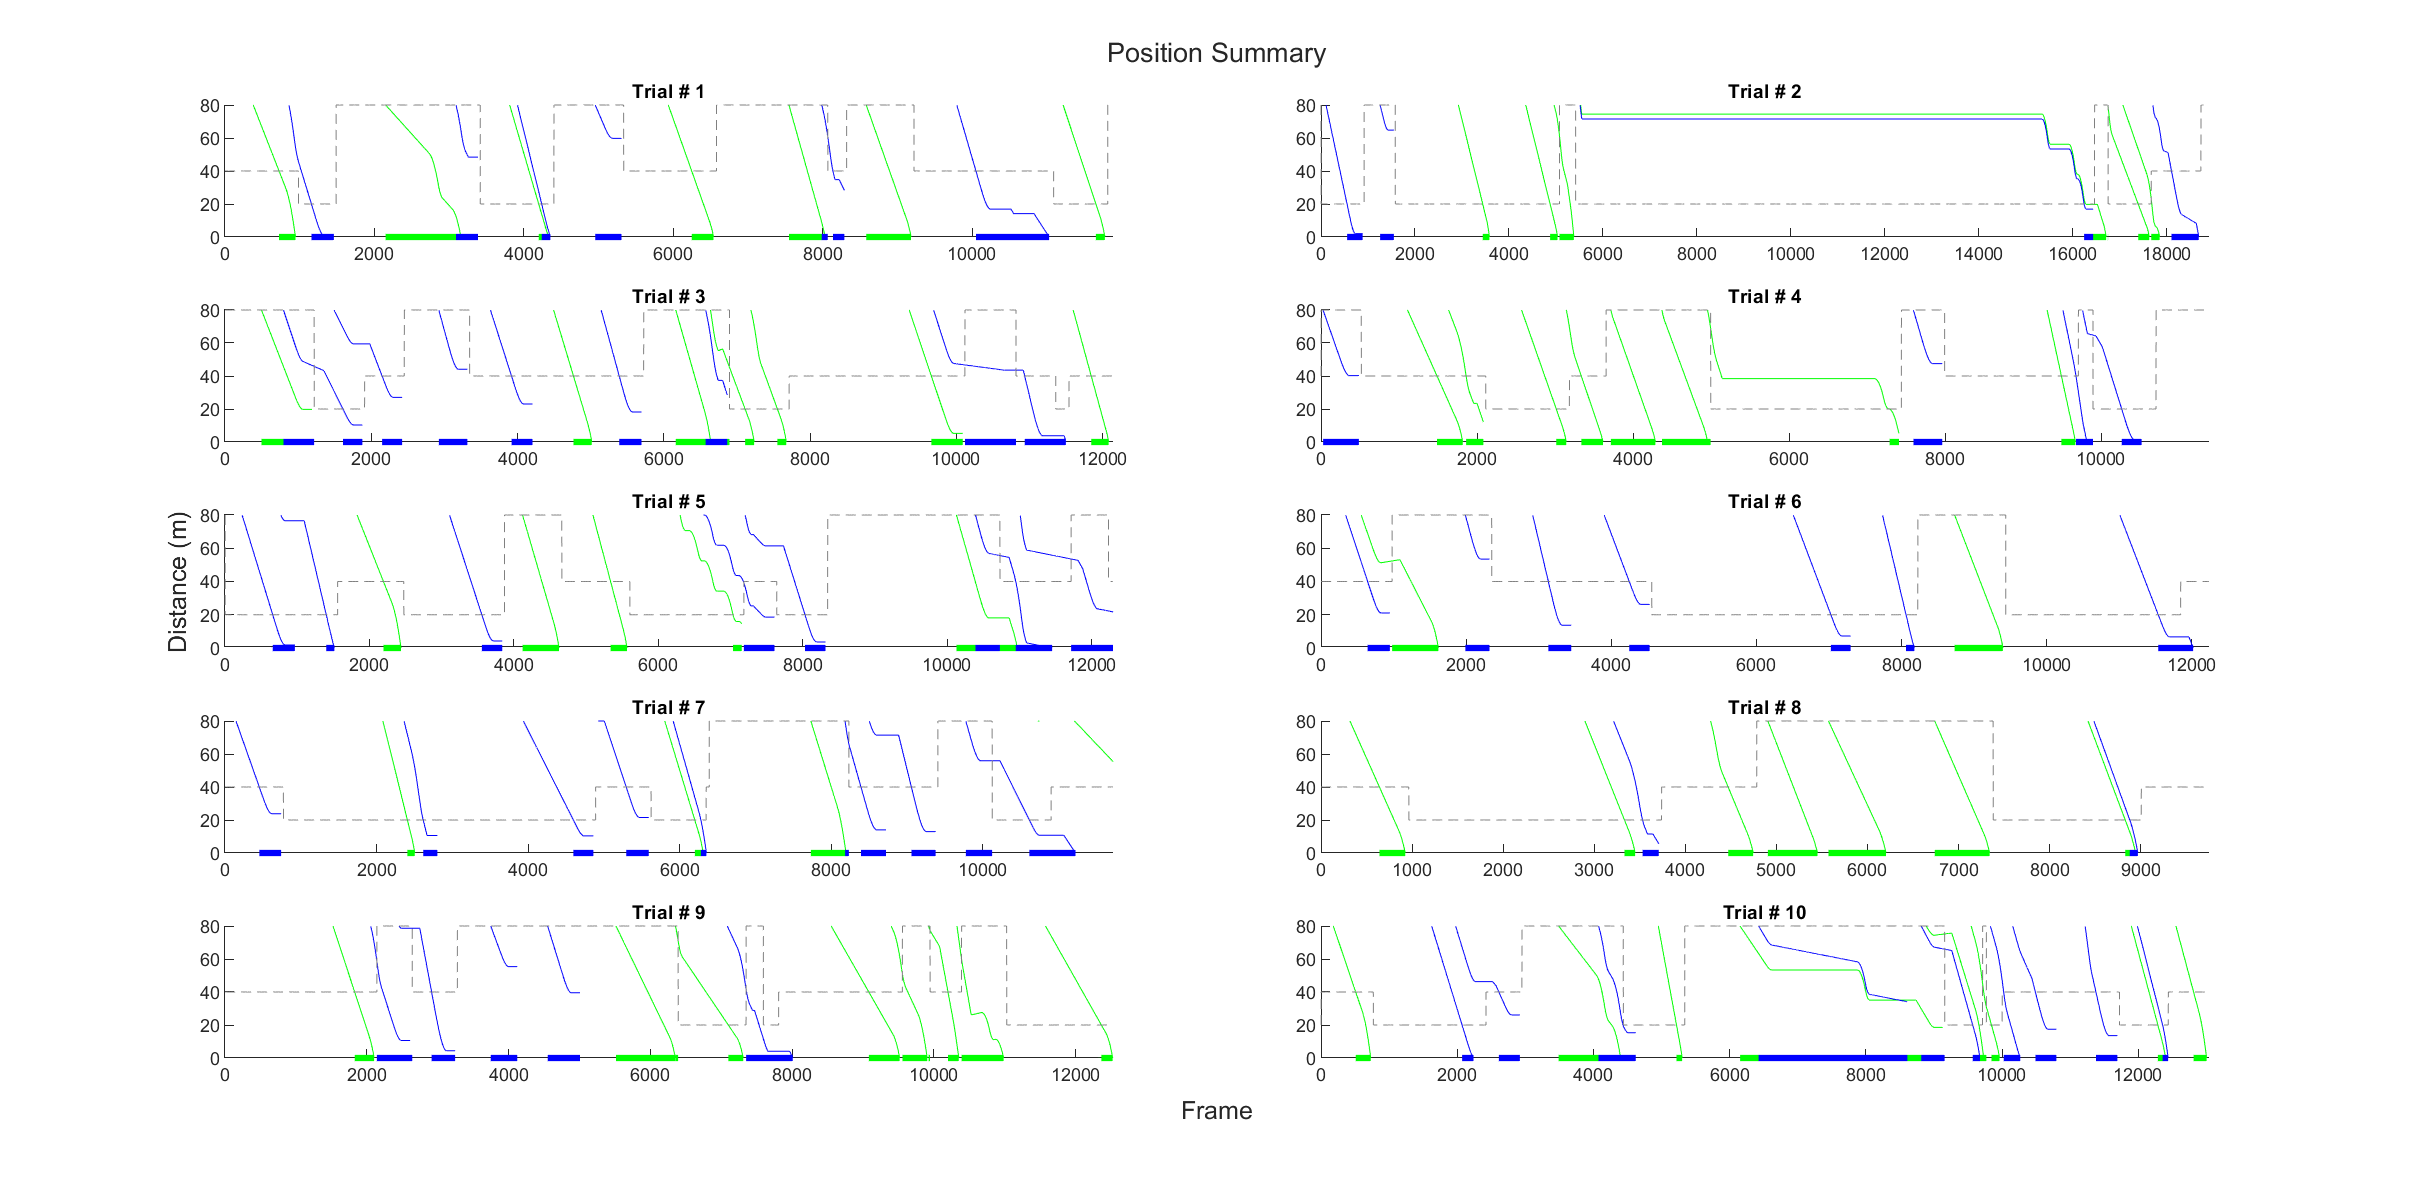
\includegraphics[width=\linewidth, height=\plotHeight\linewidth]{figures/subject_a_summary.eps}
    \caption{Summary Plot of Subject A's Trials}
    \label{fig:SumA}
\end{figure}
% Subject B
\begin{figure}[H]
    \centering
    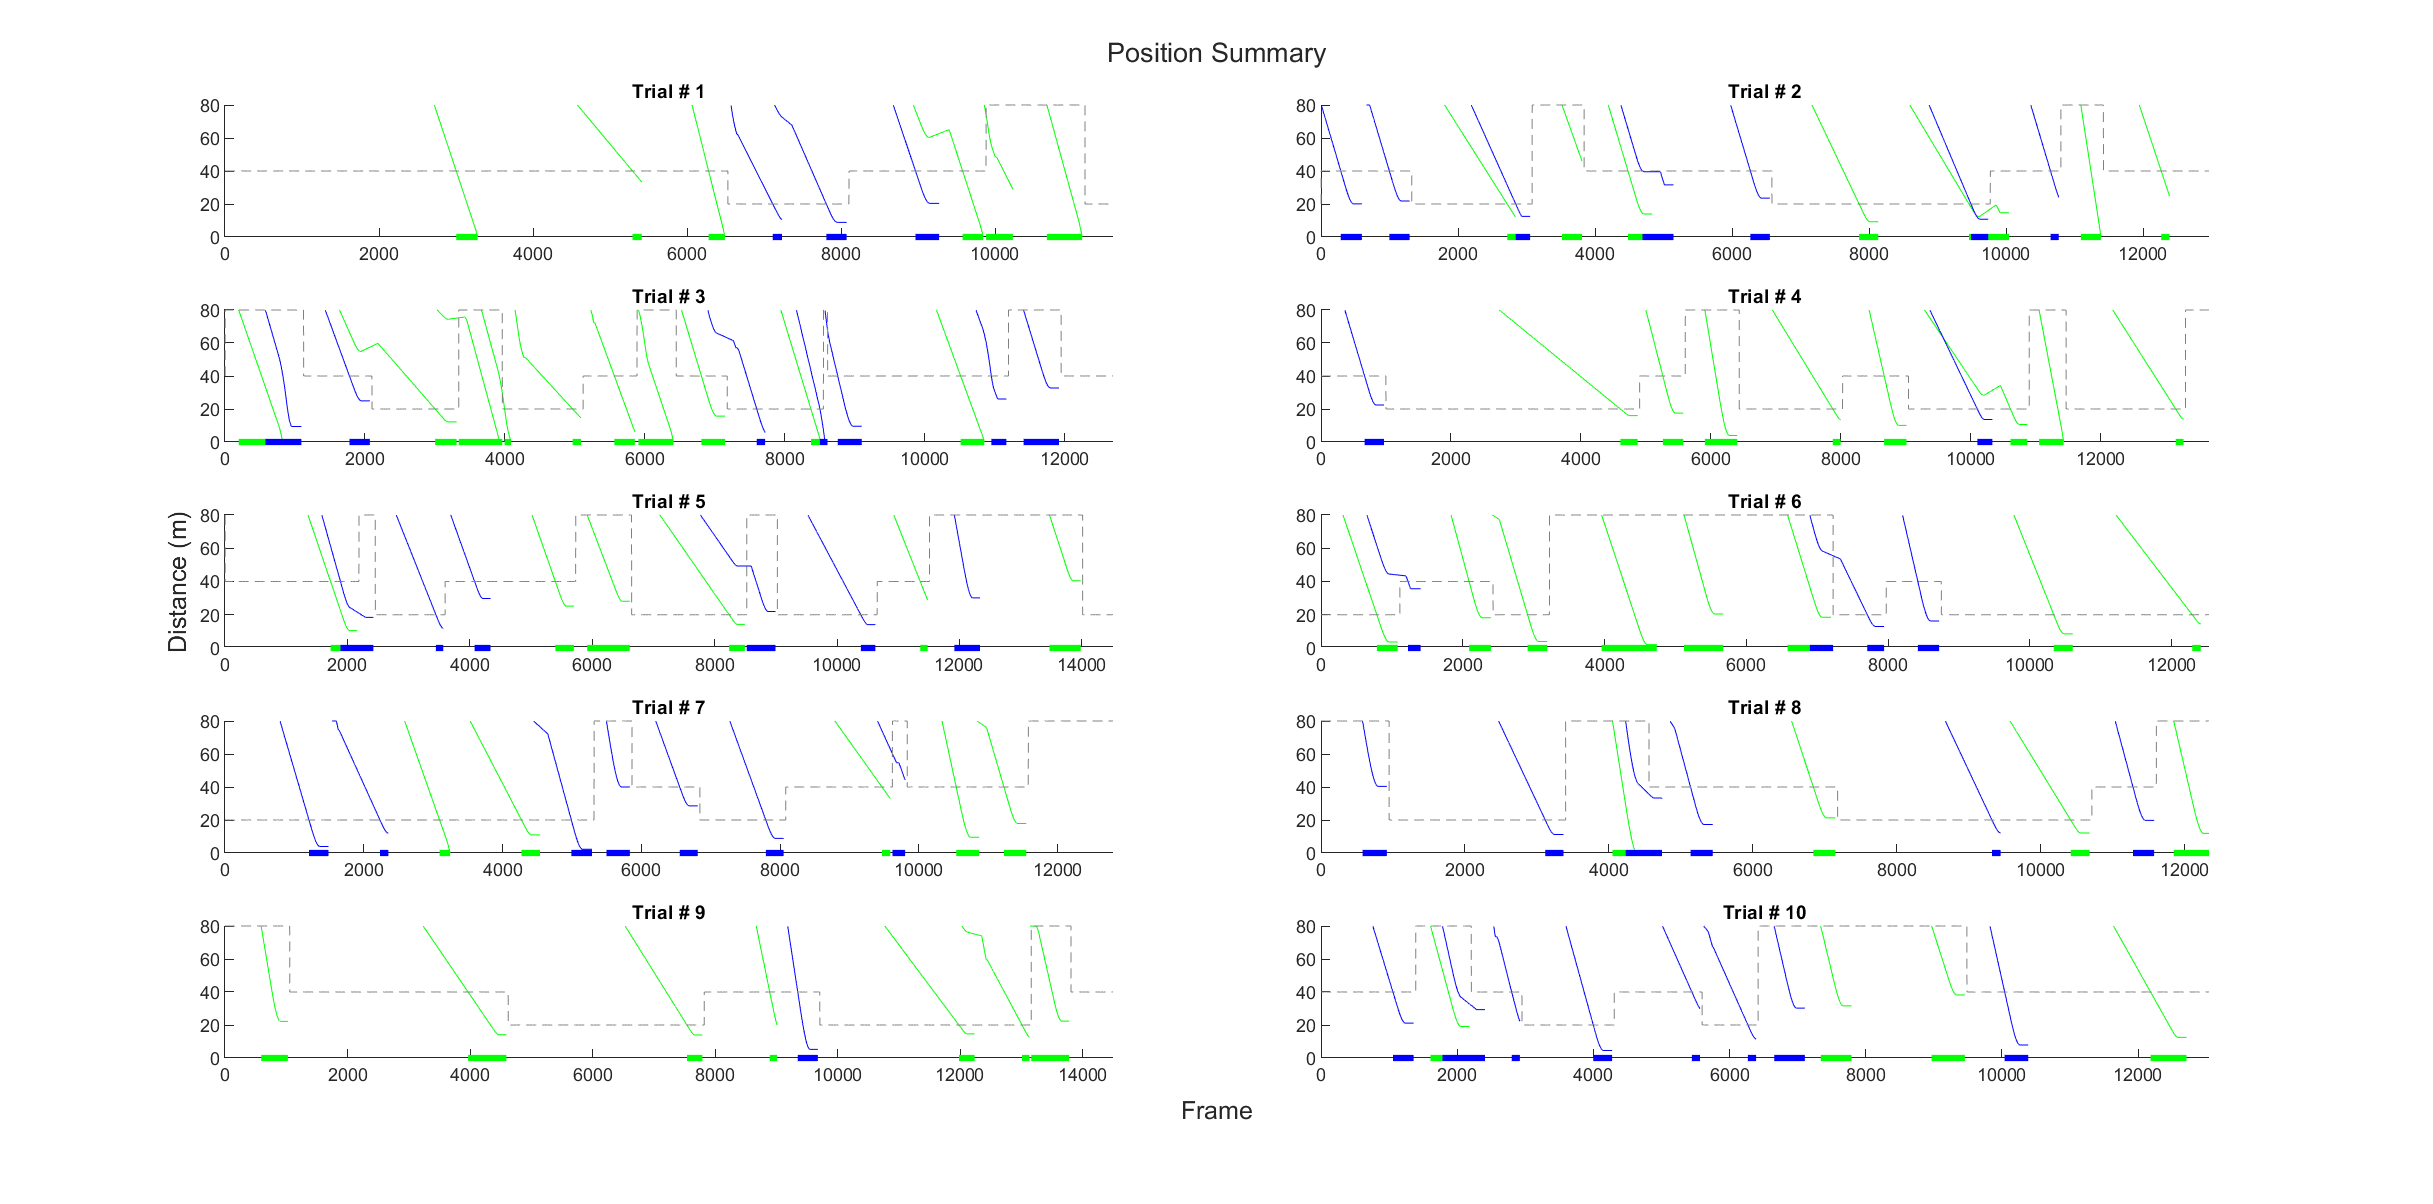
\includegraphics[width=\linewidth, height=\plotHeight\linewidth]{figures/subject_b_summary.eps}
    \caption{Summary Plot of Subject B's Trials}
    \label{fig:SumB}
\end{figure}
% Subject C
\begin{figure}[H]
    \centering
    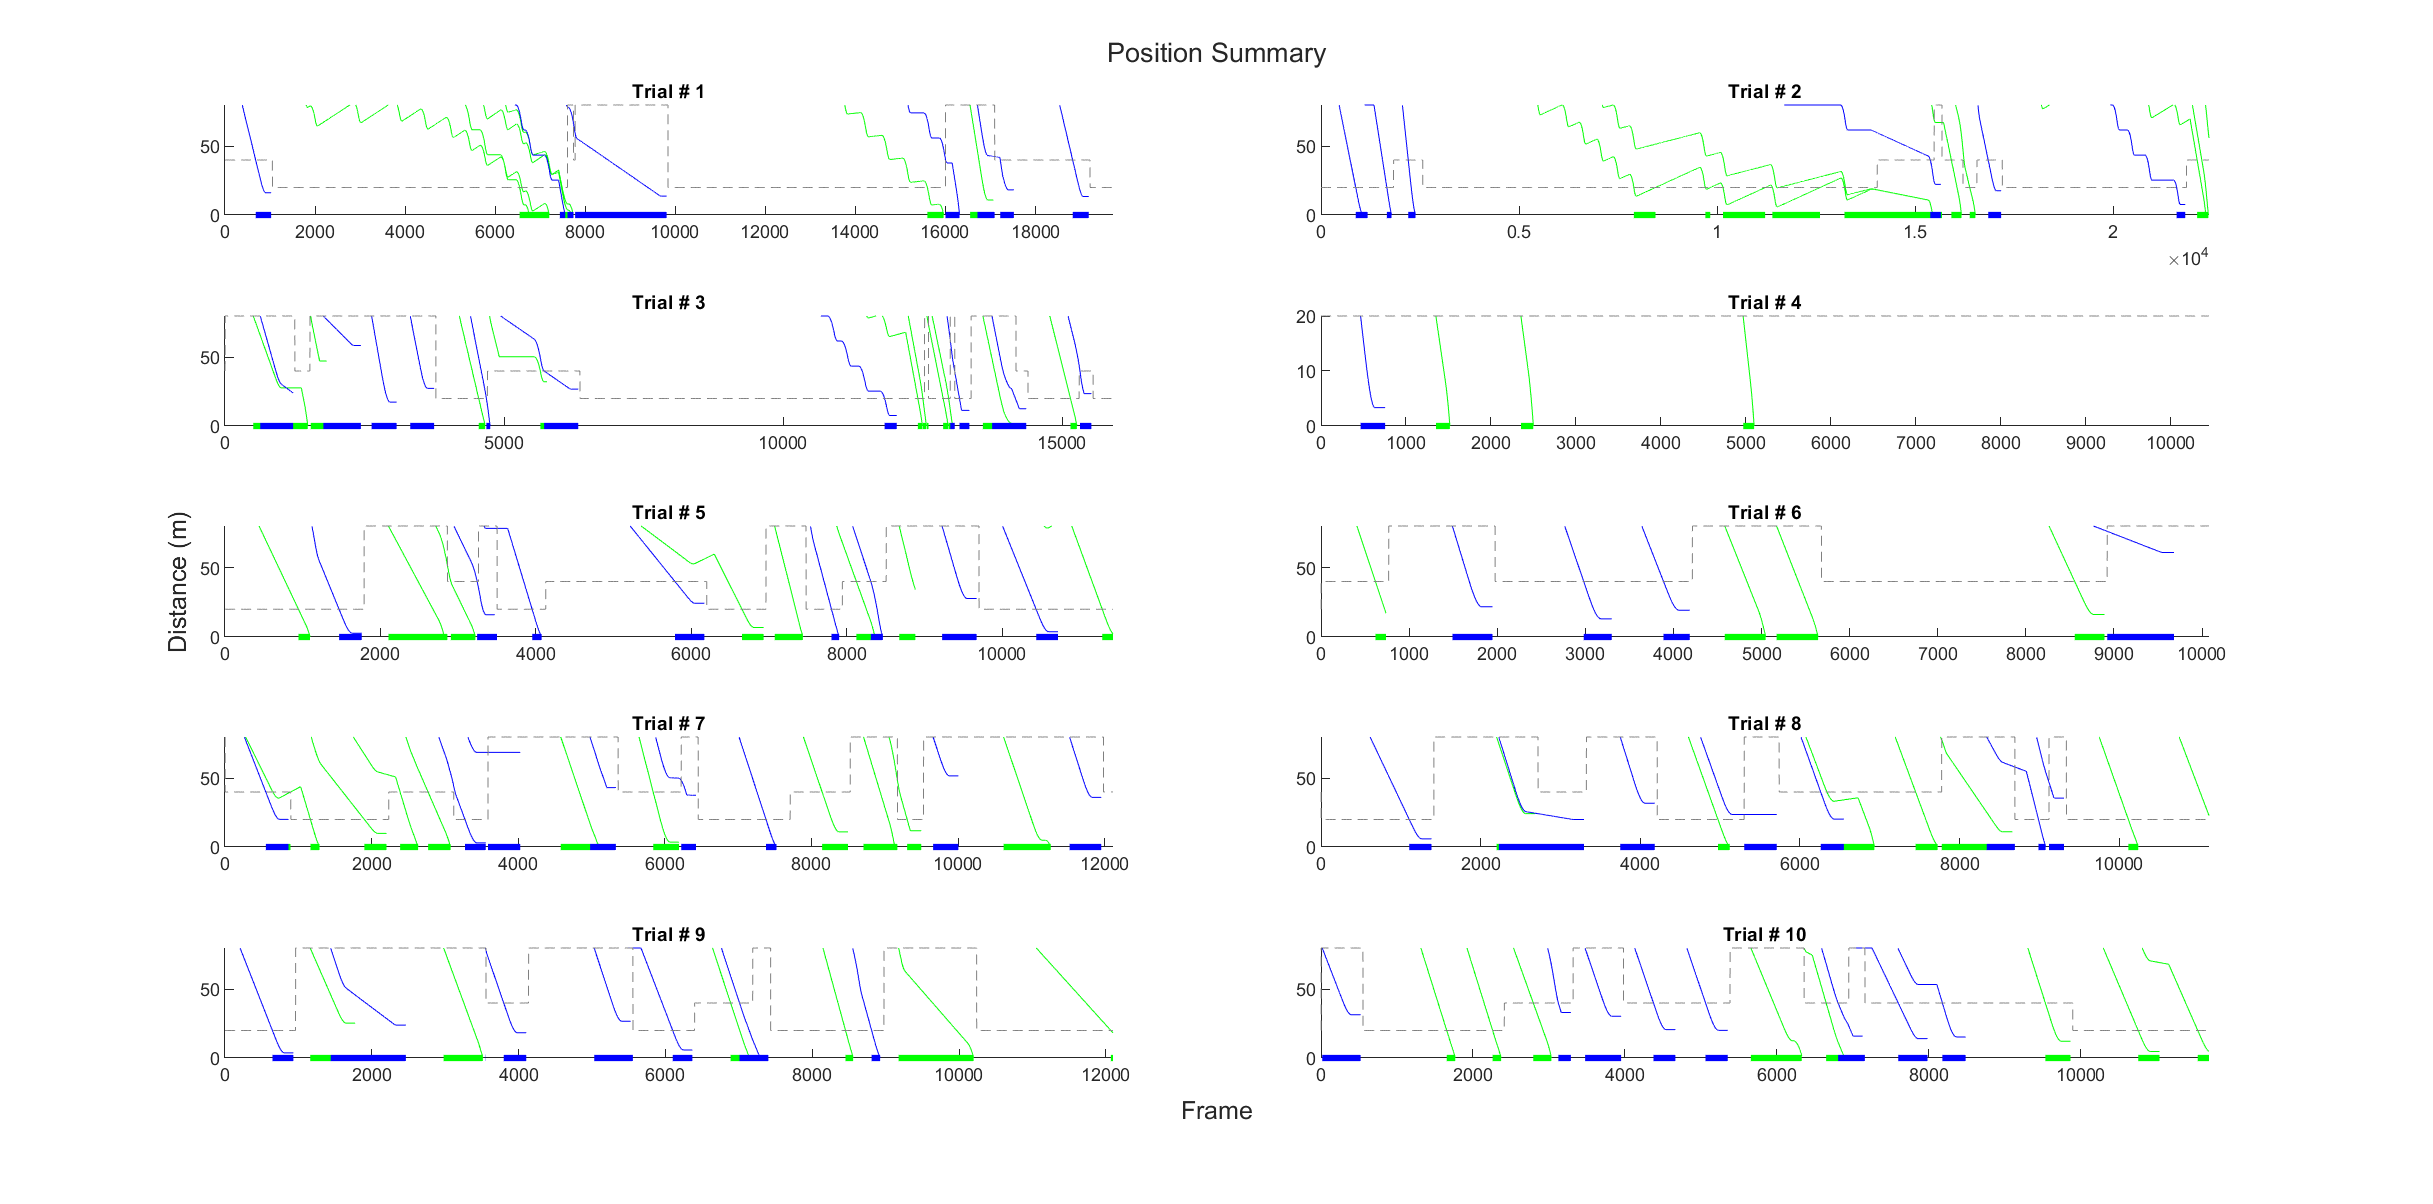
\includegraphics[width=\linewidth, height=\plotHeight\linewidth]{figures/subject_c_summary.eps}
    \caption{Summary Plot of Subject C's Trials}
    \label{fig:SumC}
\end{figure}
% Subject D
\begin{figure}[H]
    \centering
    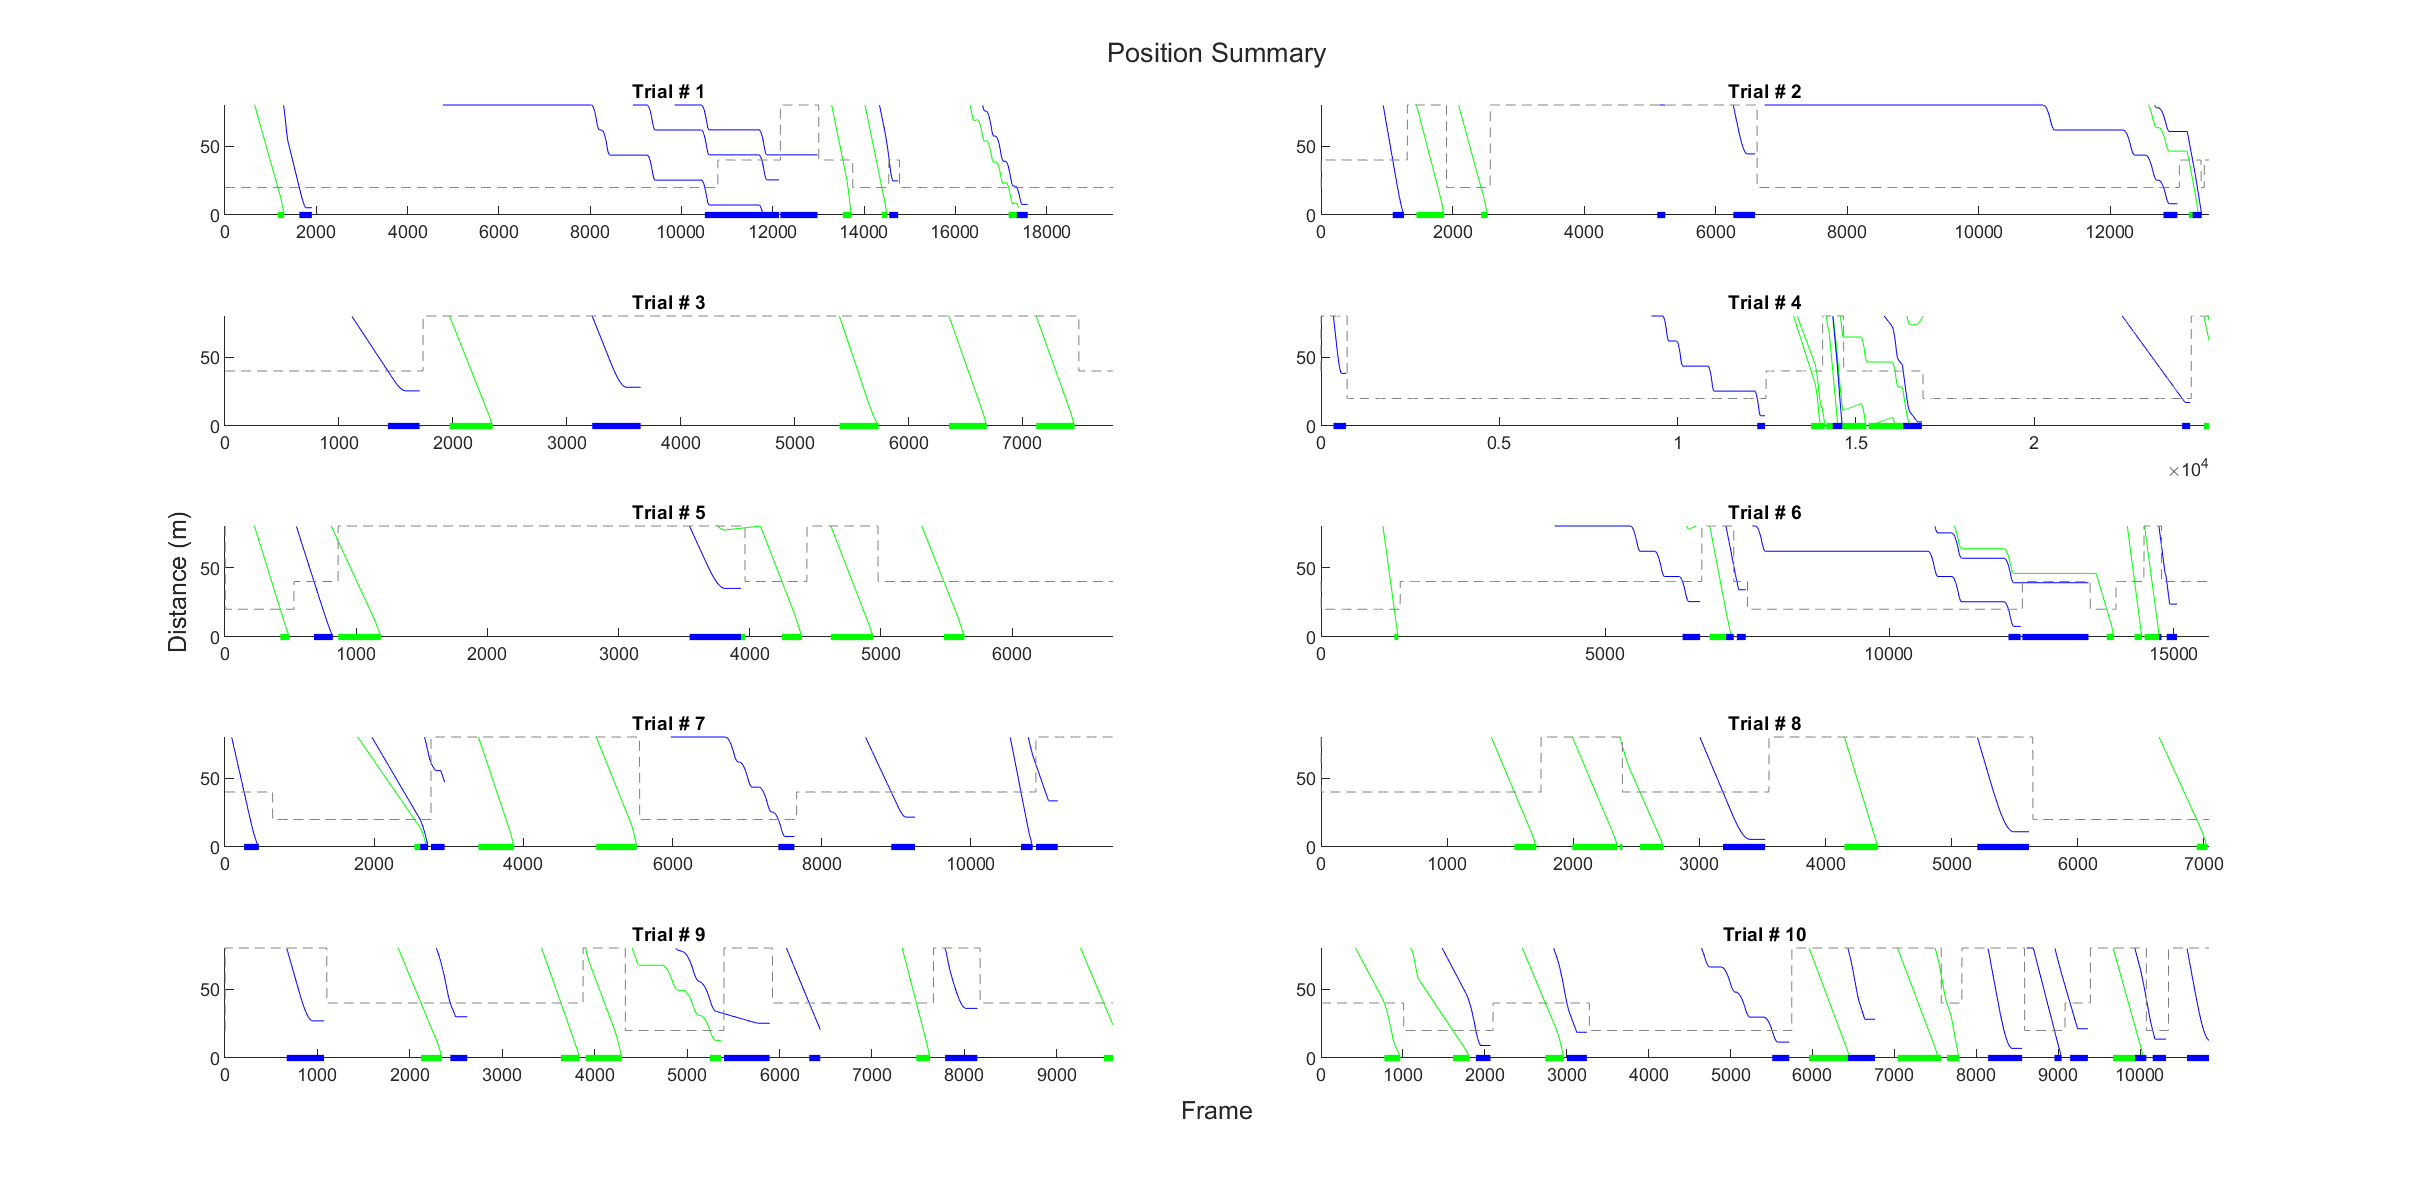
\includegraphics[width=\linewidth, height=\plotHeight\linewidth]{figures/subject_d_summary.eps}
    \caption{Summary Plot of Subject D's Trials}
    \label{fig:SumD}
\end{figure}
% Subject E
\begin{figure}[H]
    \centering
    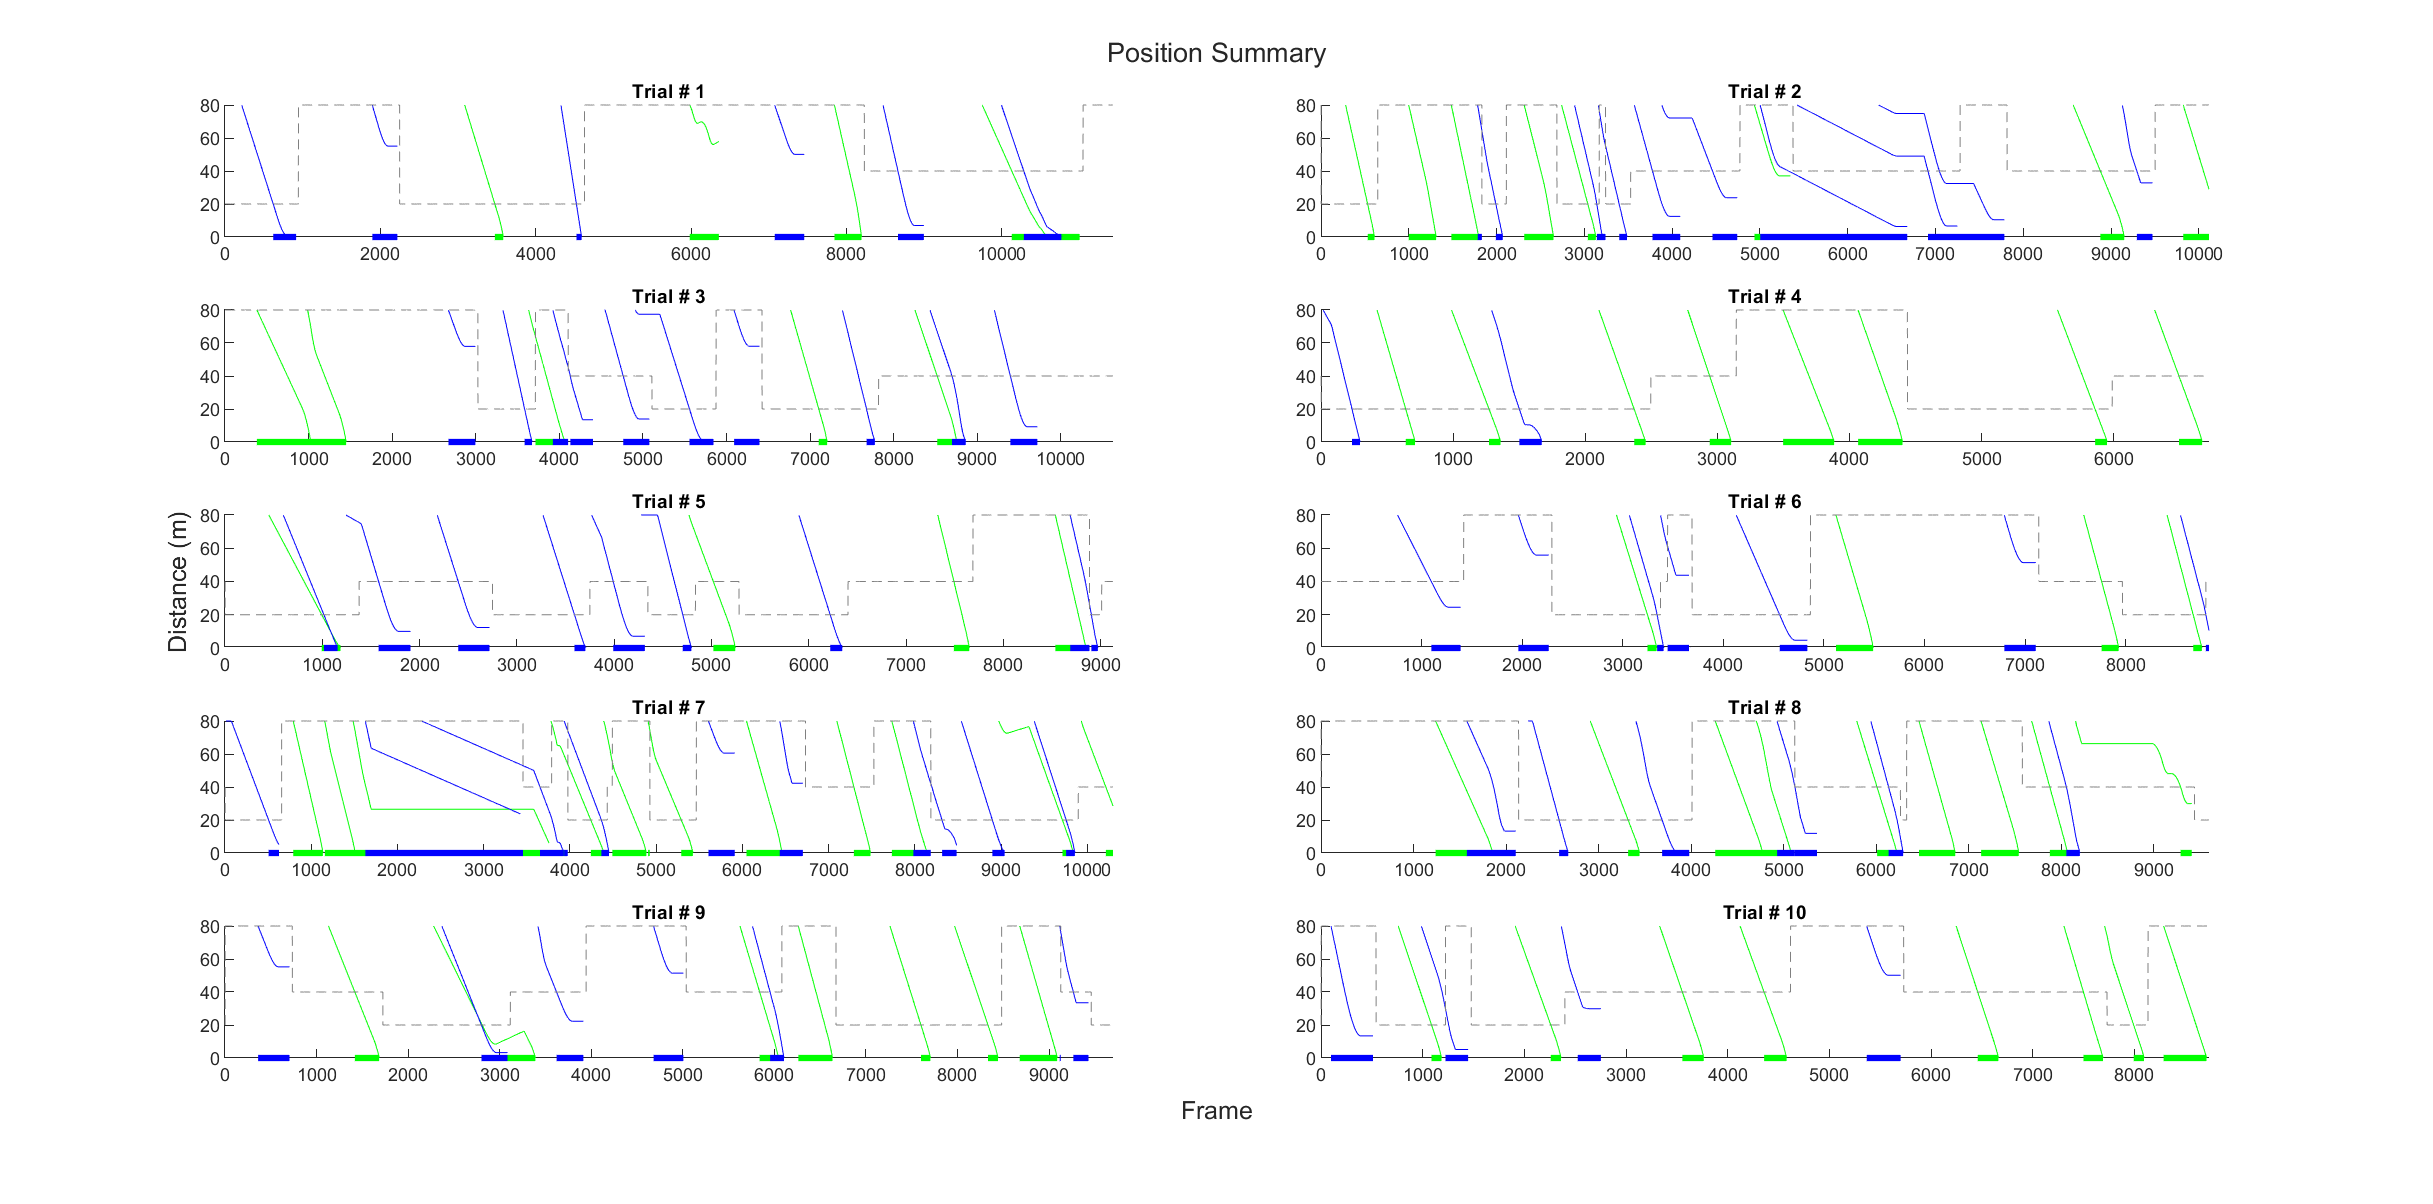
\includegraphics[width=\linewidth, height=\plotHeight\linewidth]{figures/subject_e_summary.eps}
    \caption{Summary Plot of Subject E's Trials}
    \label{fig:SumE}
\end{figure}
% Subject F
\begin{figure}[H]
    \centering
    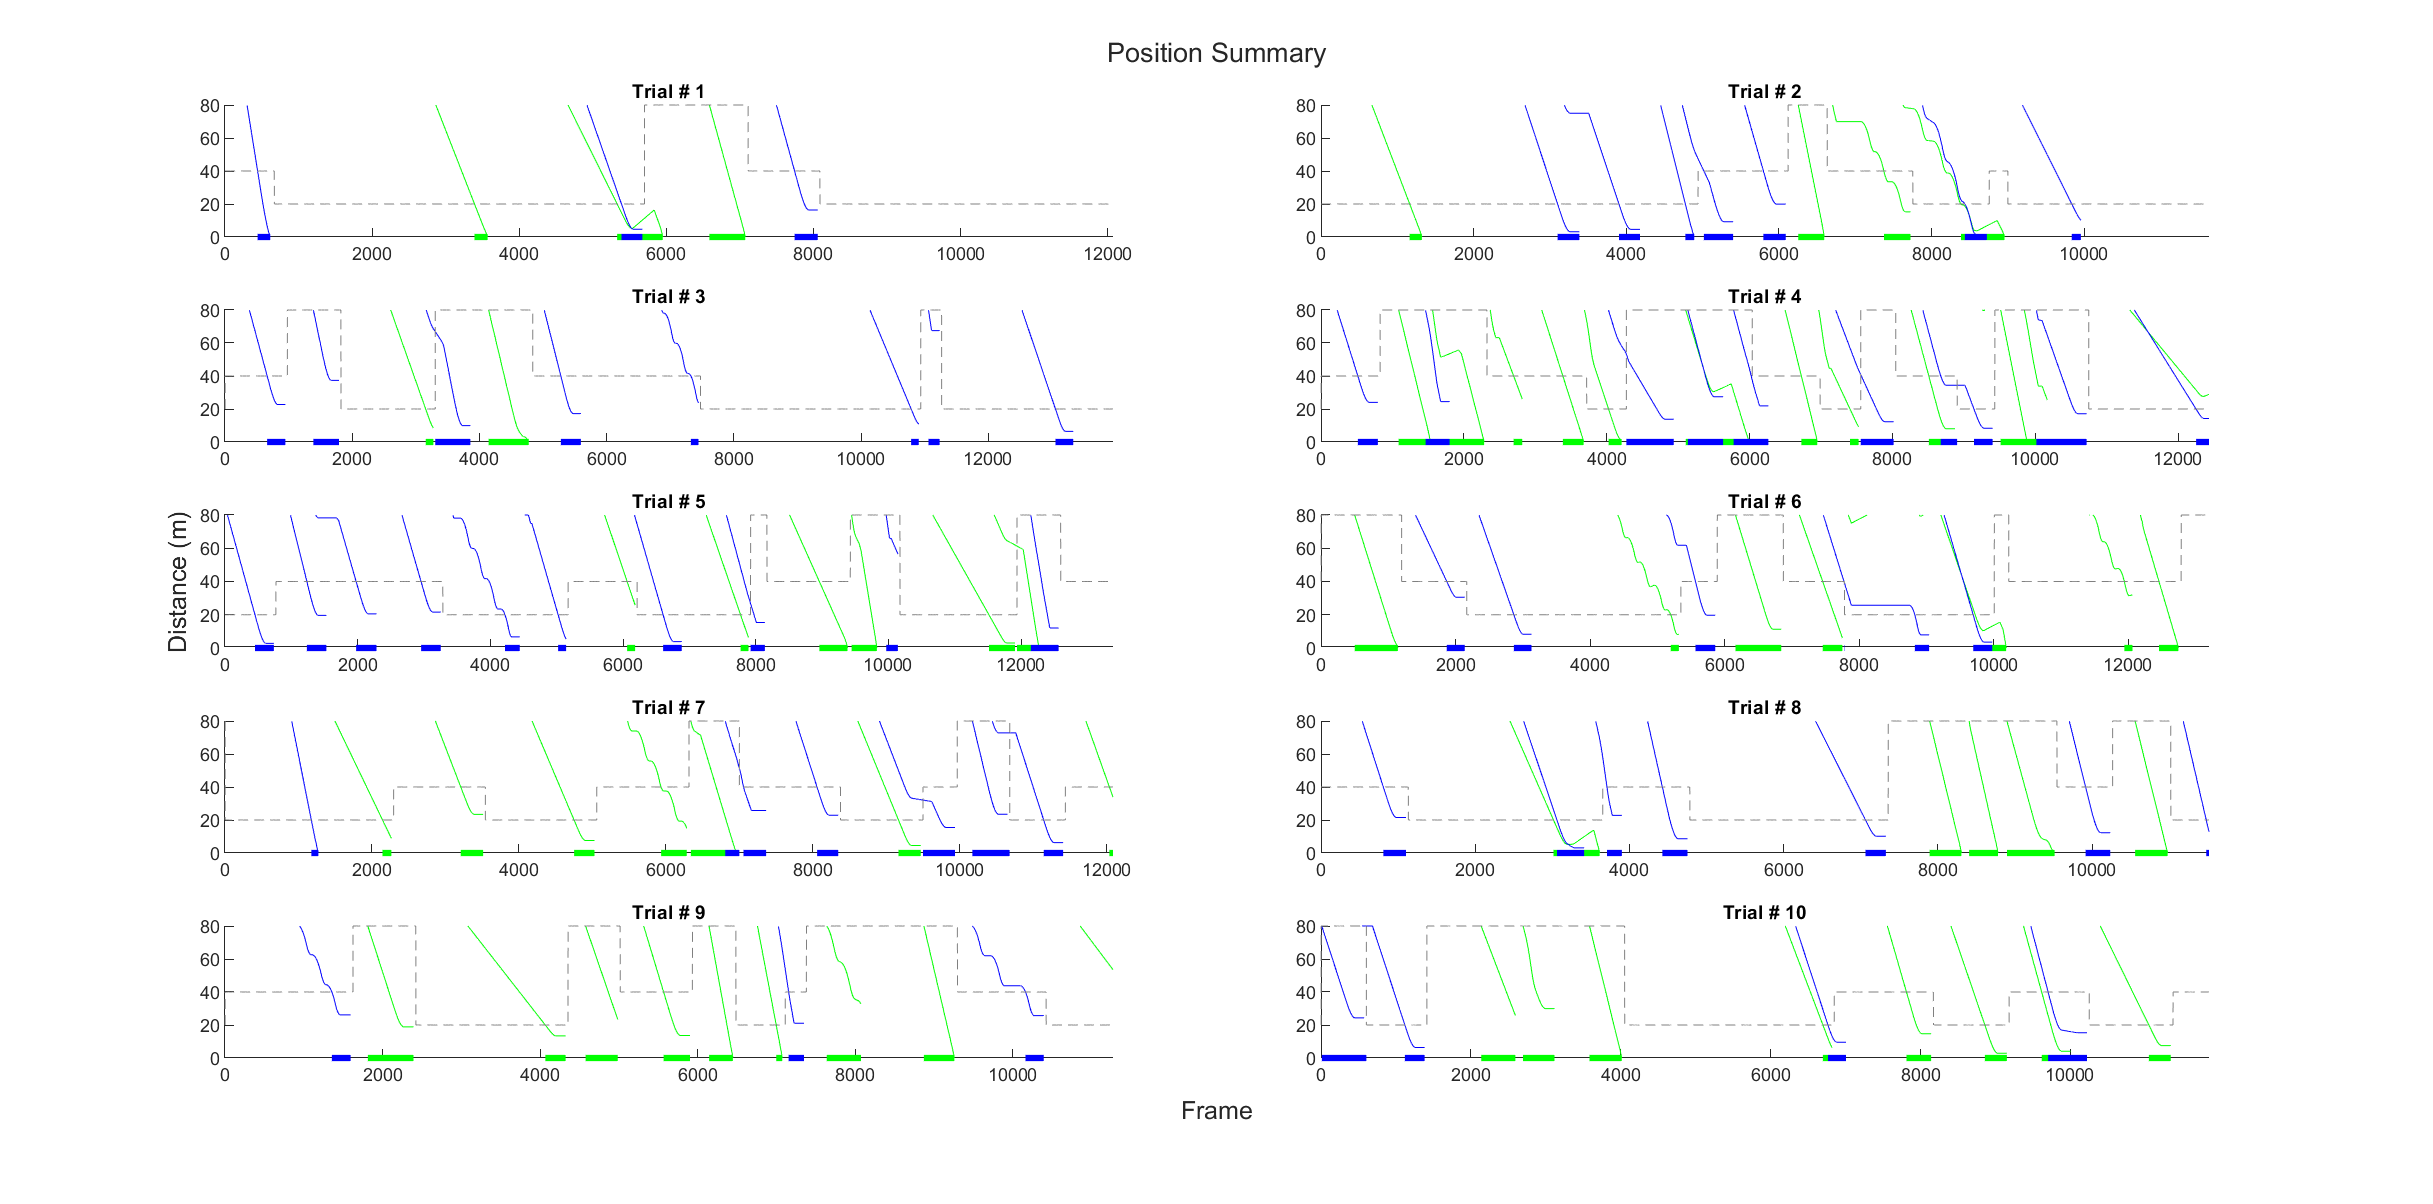
\includegraphics[width=\linewidth, height=\plotHeight\linewidth]{figures/subject_f_summary.eps}
    \caption{Summary Plot of Subject F's Trials}
    \label{fig:SumF}
\end{figure}

% ----------------------
% This is the second section, reaction times by subject
\section{Response Summary Plots by Subject}
\label{appendix:ExtraResults0_2}
\subsection{Response Times to Cyclist Stimuli}
\begin{figure}[H]
    \centering
    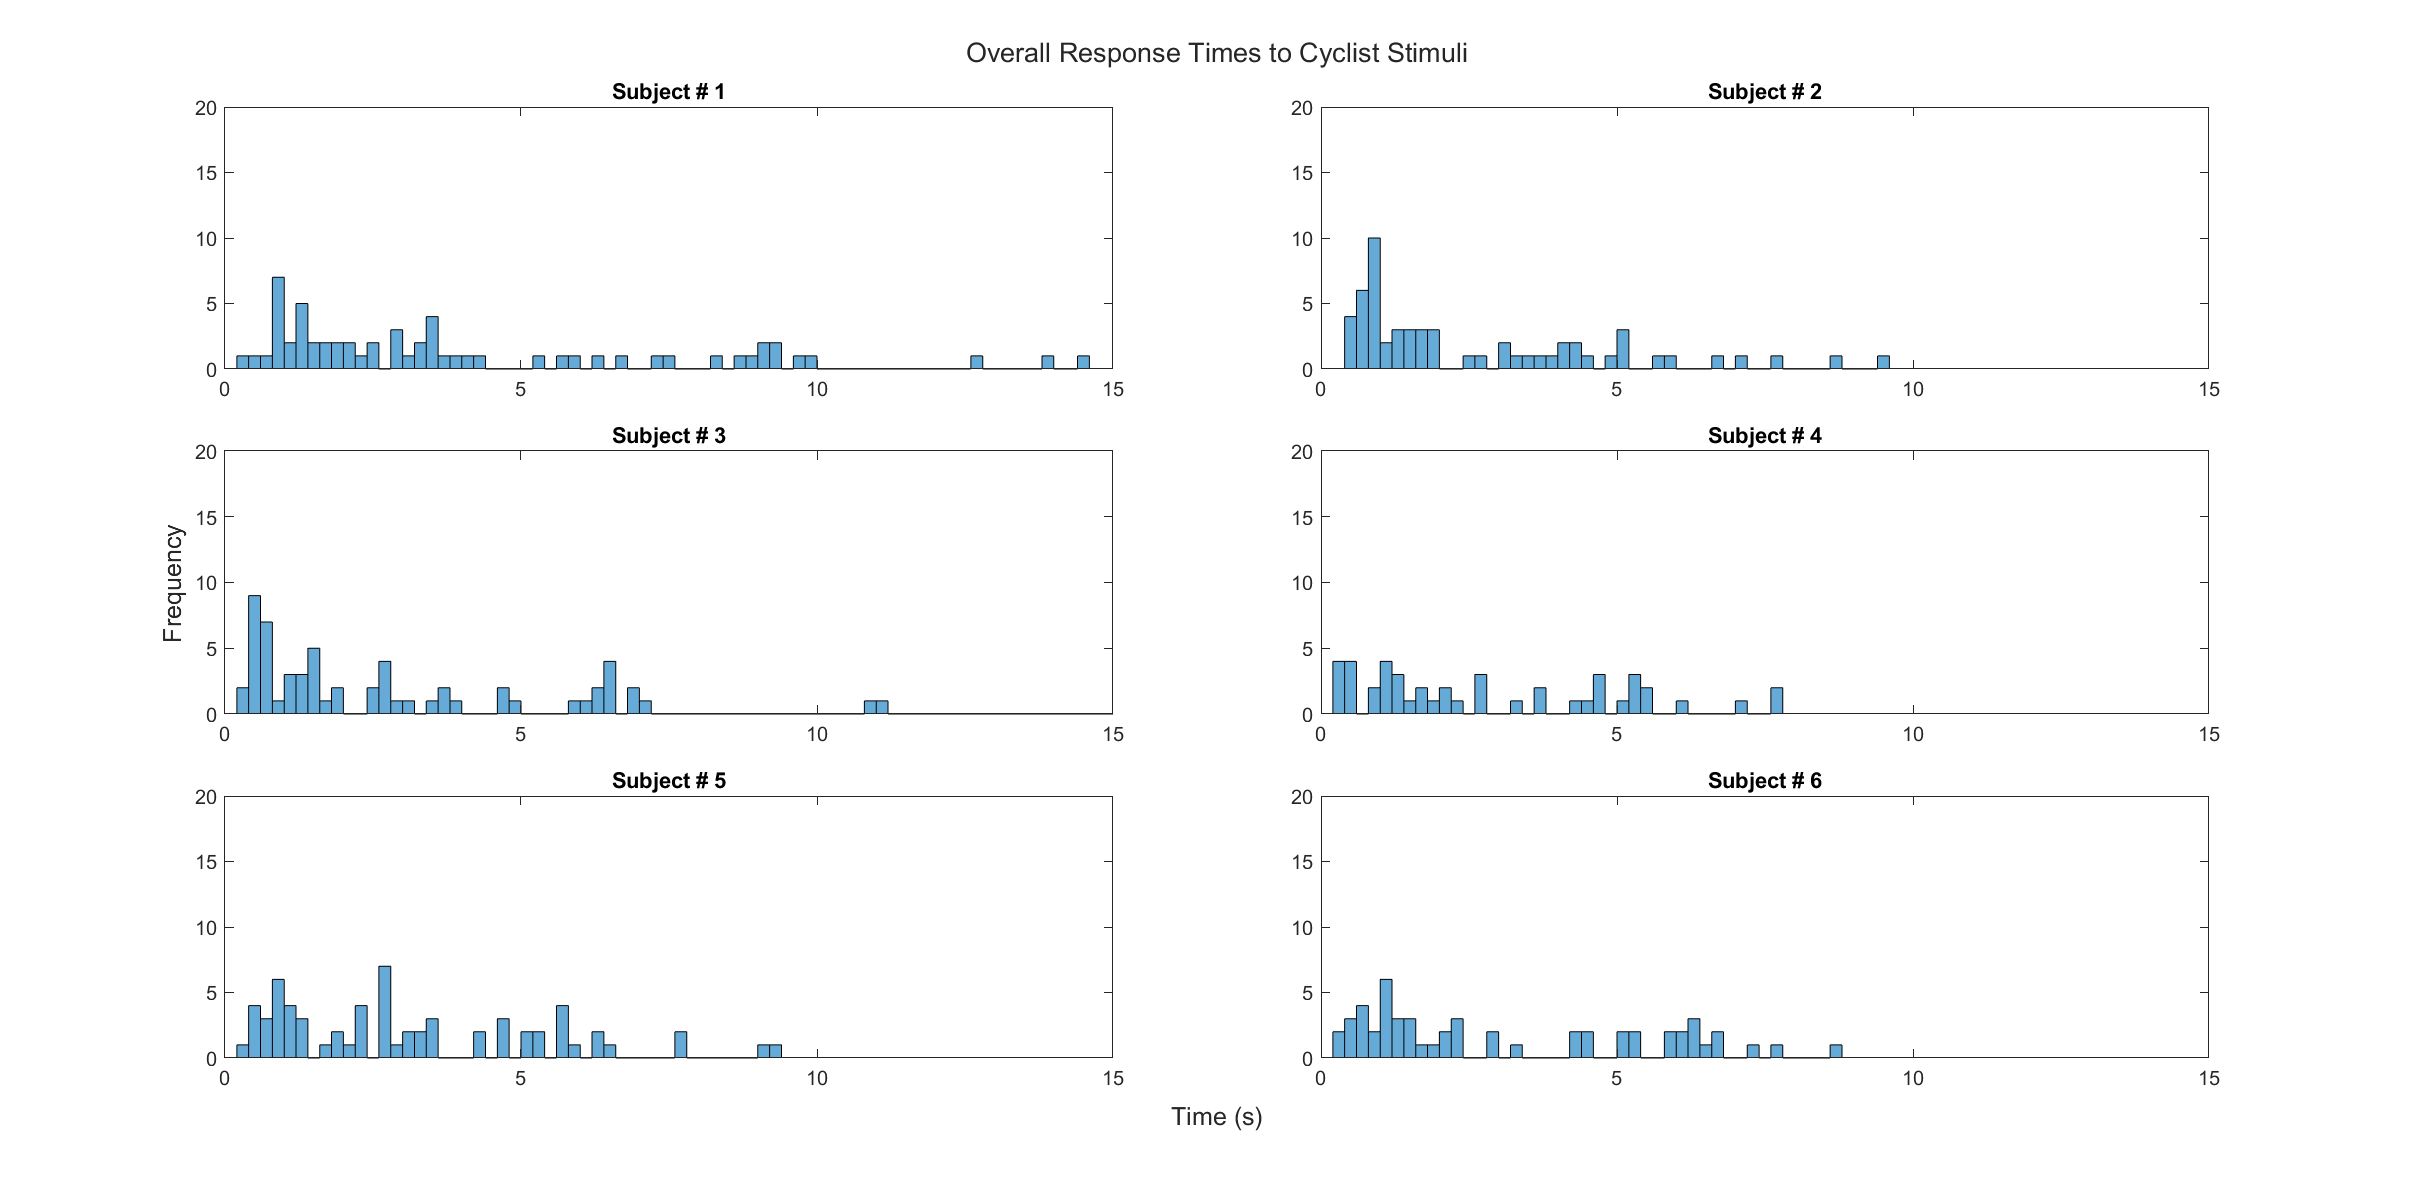
\includegraphics[width=\linewidth, height=\plotHeight\linewidth]{figures/BikeReactionTimes_by_sub.eps}
    \caption{Summary Plot of Response Times to the Cyclist Stimuli by Subject No Distinction by Decision Made}
    \label{fig:RT_B_1bysub}
\end{figure}
\begin{figure}[H]
    \centering
    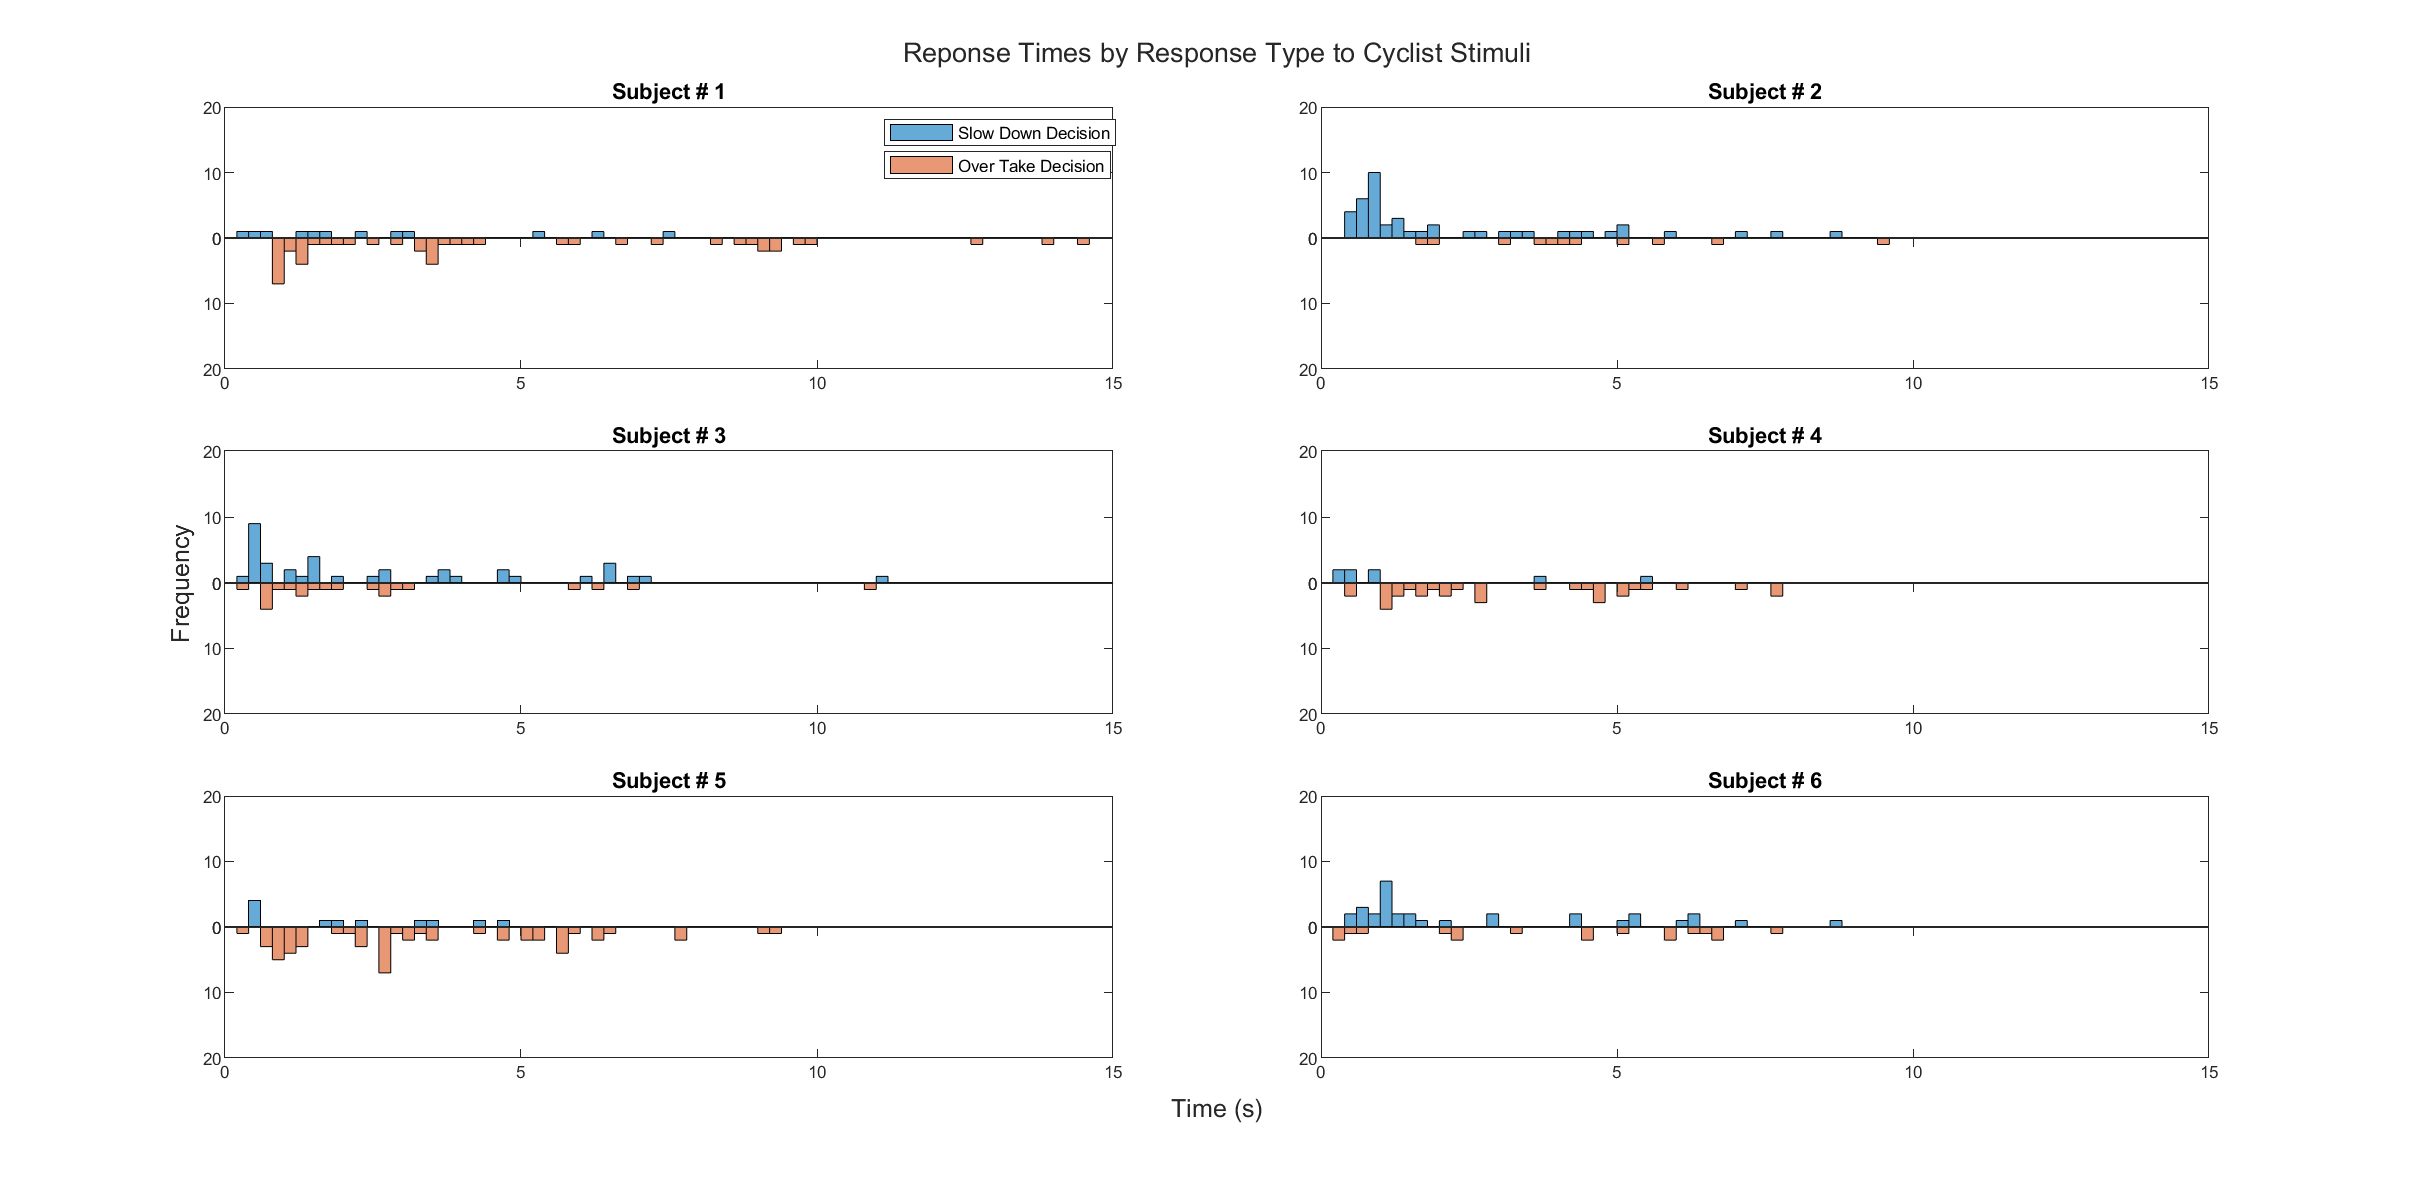
\includegraphics[width=\linewidth, height=\plotHeight\linewidth]{figures/BikeReactionTimes2_by_sub.eps}
    \caption{Summary Plot of Response Times to the Bike Stimuli by Subject Disaggregated by Decision Made}
    \label{fig:RT_B_2bysub}
\end{figure}

\subsection{Response Times to Car Stimuli}
\begin{figure}[H]
    \centering
    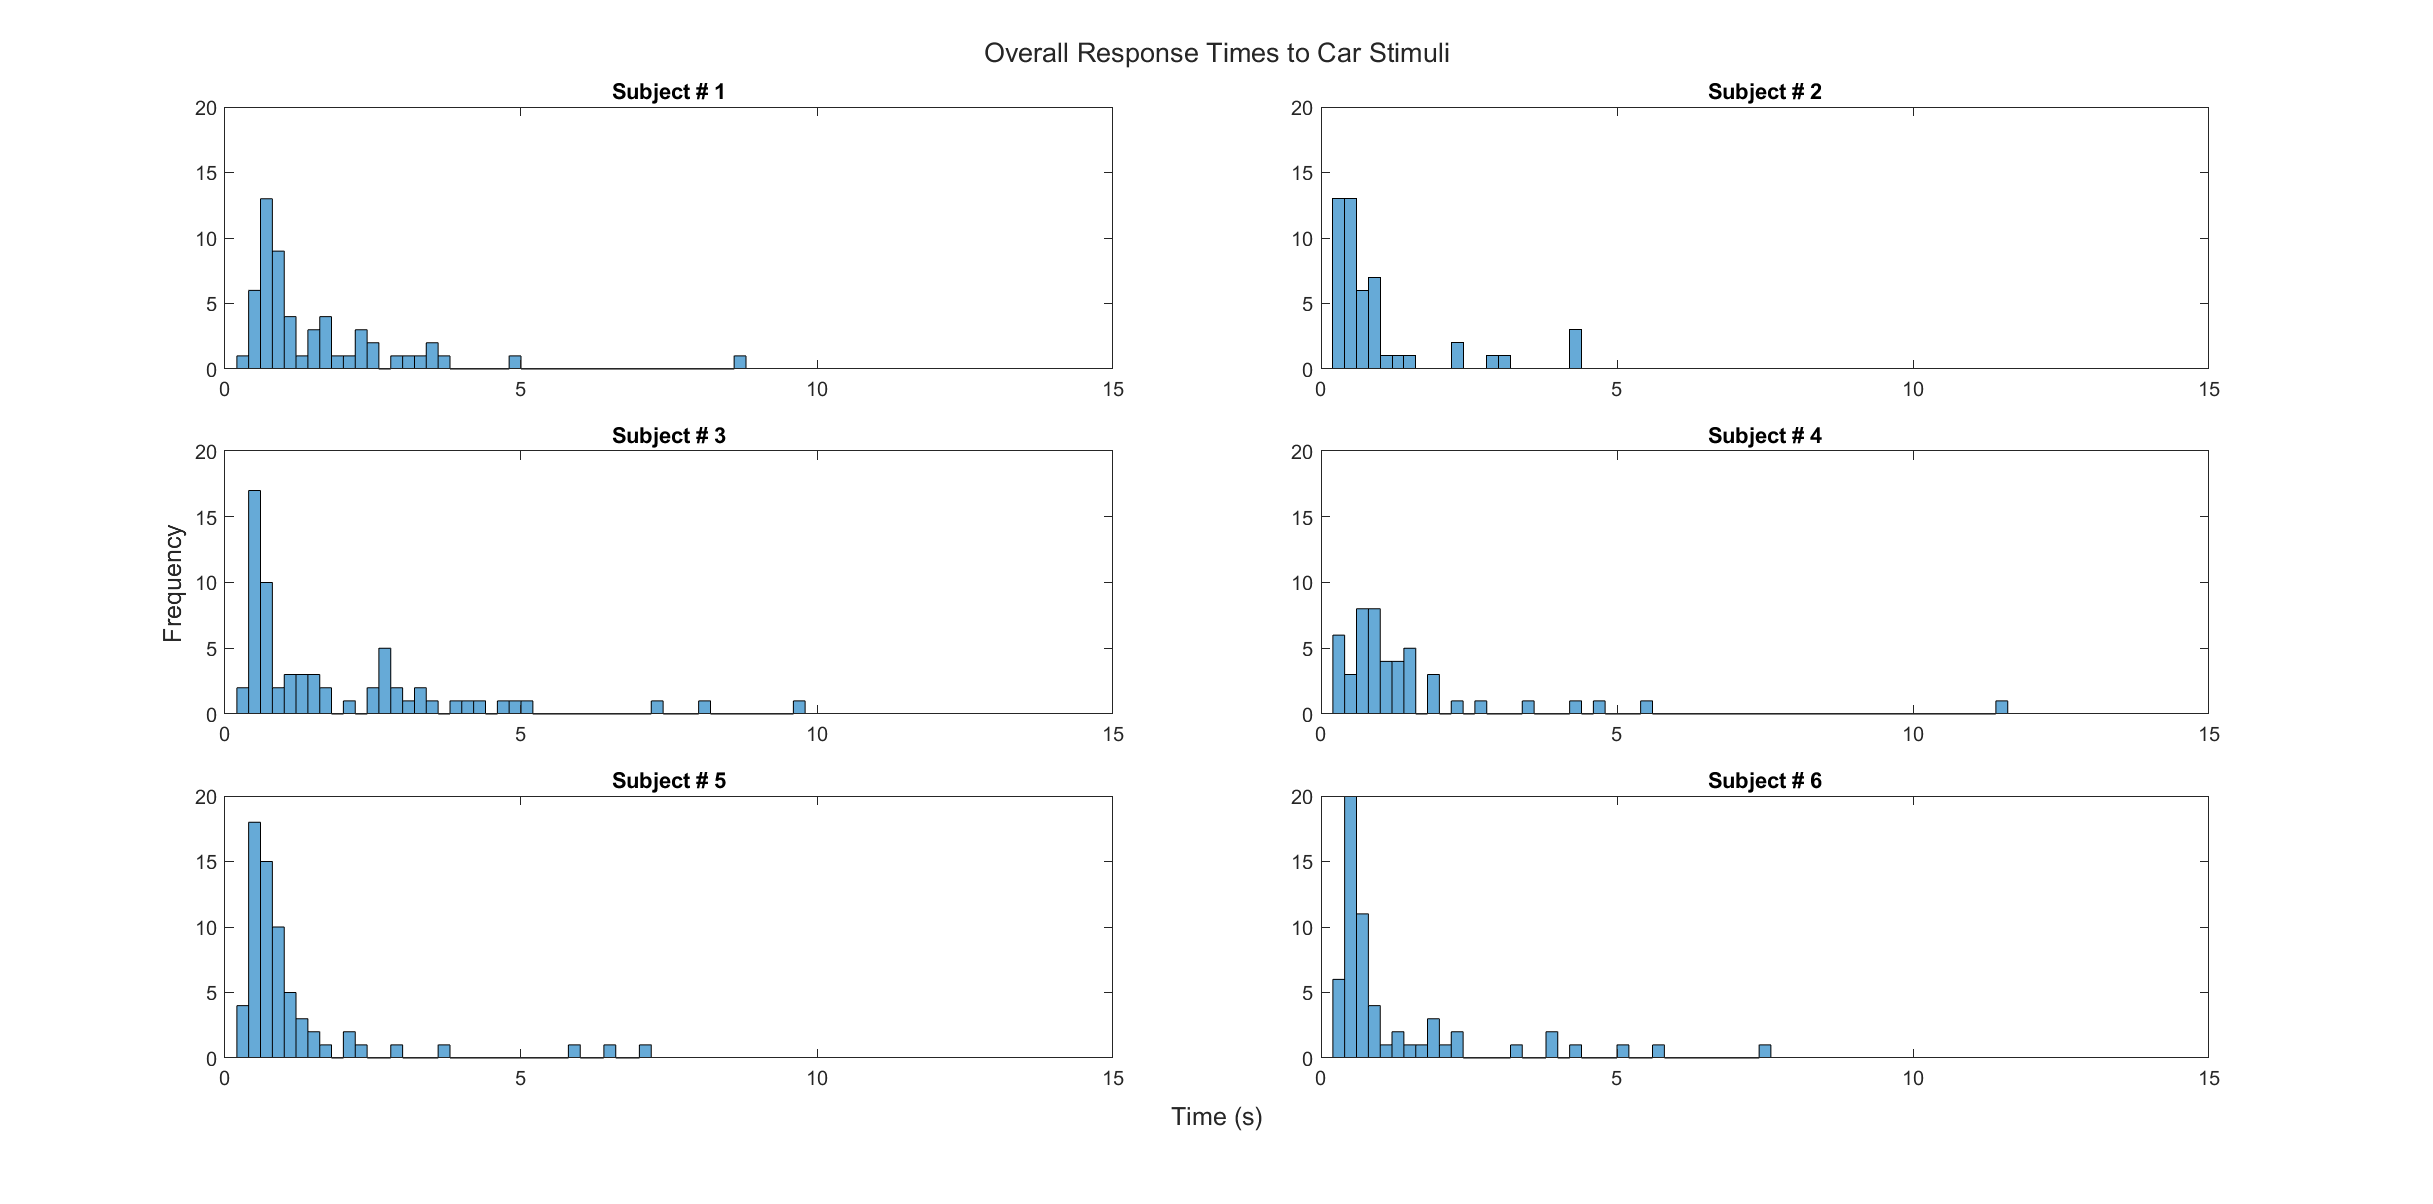
\includegraphics[width=\linewidth, height=\plotHeight\linewidth]{figures/CarReactionTimes_by_sub.eps}
    \caption{Summary Plot of Response Times to the Car Stimuli by Subject No Distinction by Decision Made}
    \label{fig:RT_C_1bysub}
\end{figure}
\begin{figure}[H]
    \centering
    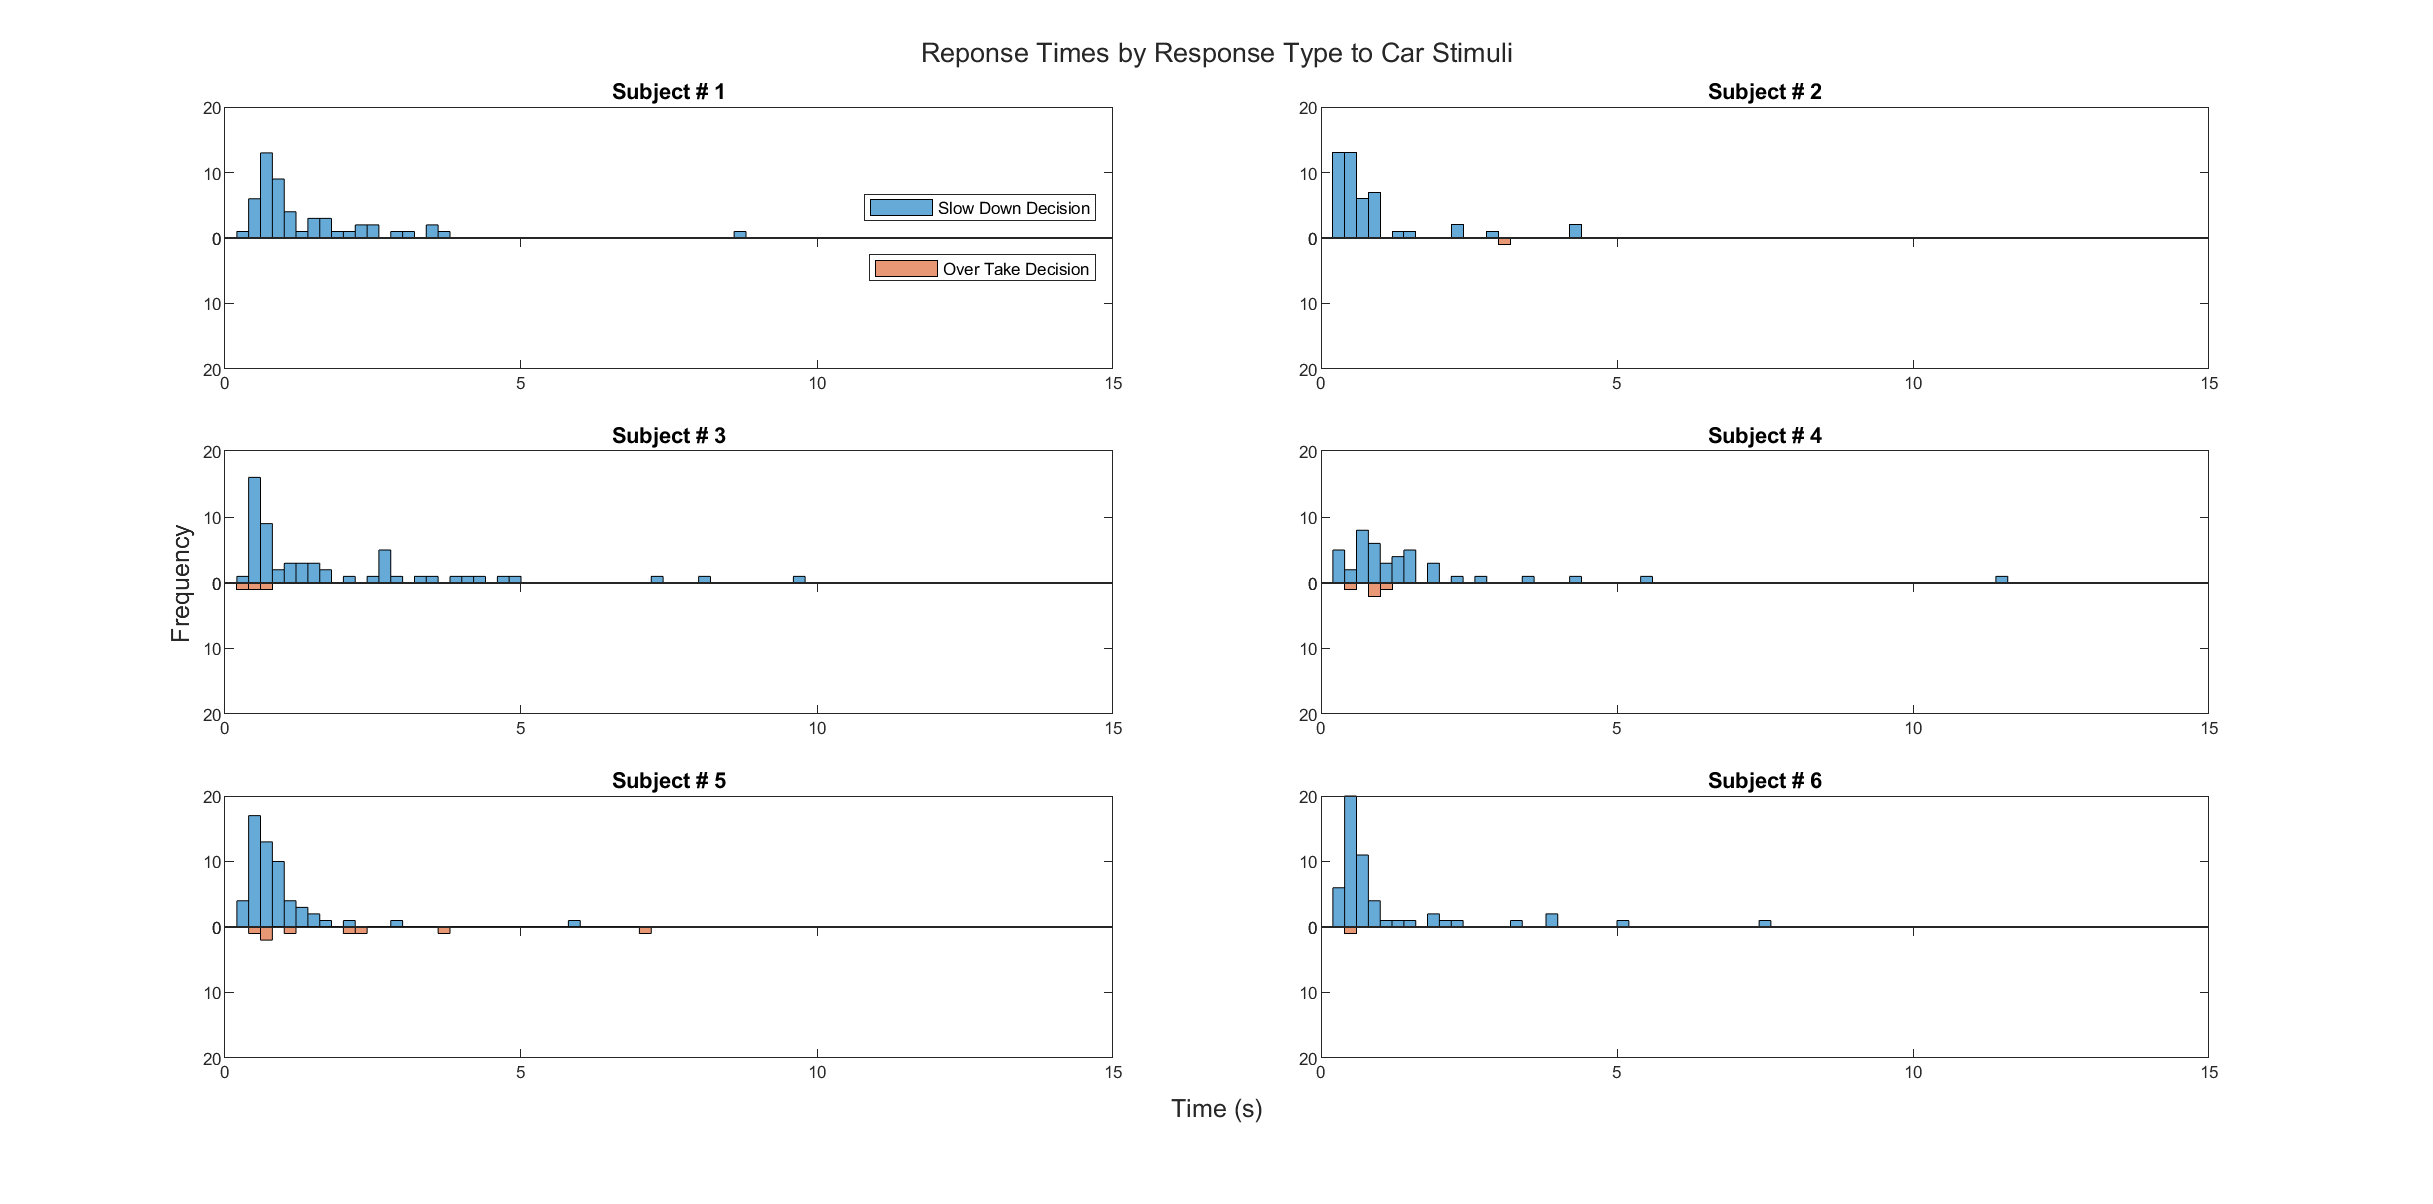
\includegraphics[width=\linewidth, height=\plotHeight\linewidth]{figures/CarReactionTimes2_by_sub.eps}
    \caption{Summary Plot of Response Times to the Car Stimuli by Subject Disaggregated by Decision Made}
    \label{fig:RT_C_2bysub}
\end{figure}


%%%%%%%%%%%%
% Appendix III
%%%%%%%%%%%%
\chapter{Additional EMG Results}
\label{appendix:ExtraResults1}
Note: Subject A did not have EMG recorded during their trial. As a result the appendix starts with subject B.

\section{EMG Summary Plots}
\label{appendix:ExtraResults1_1}
\begin{figure}[H]
    \centering
    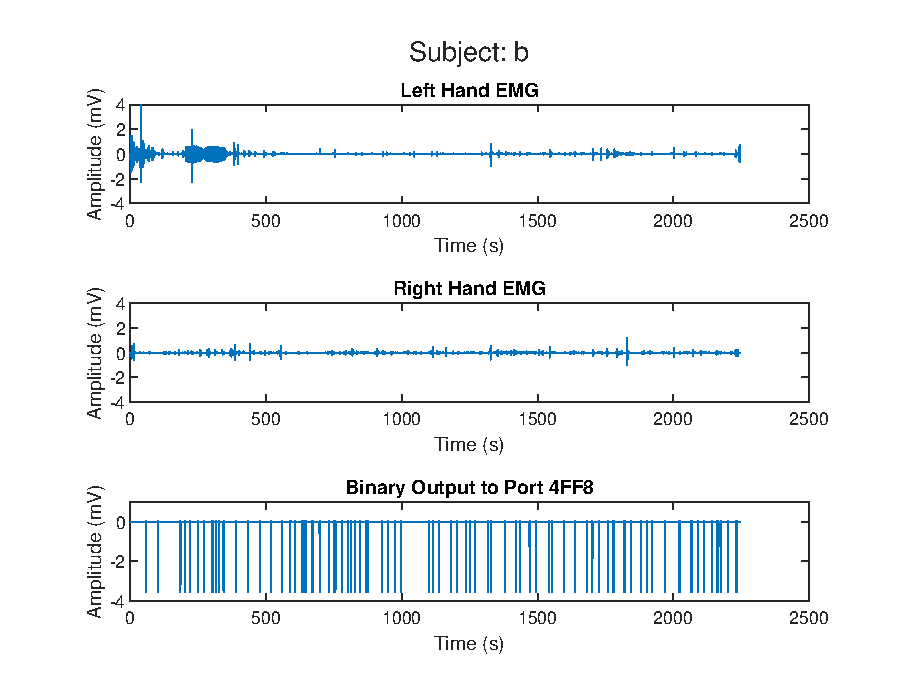
\includegraphics[width=0.75\linewidth]{figures/EMG_summary_b.eps}
    \caption{EMG Traces From Subject B's Trials}
    \label{fig:EMG_Sum_B}
\end{figure}
\begin{figure}[H]
    \centering
    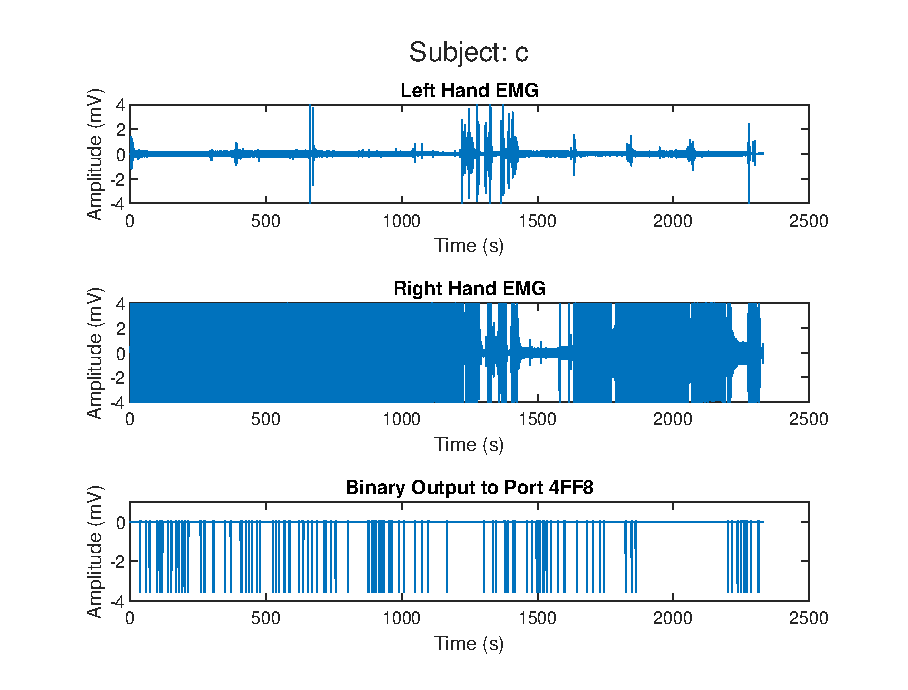
\includegraphics[width=0.75\linewidth]{figures/EMG_summary_c.eps}
    \caption{EMG Traces From Subject C's Trials}
    \label{fig:EMG_Sum_C}
\end{figure}
\begin{figure}[H]
    \centering
    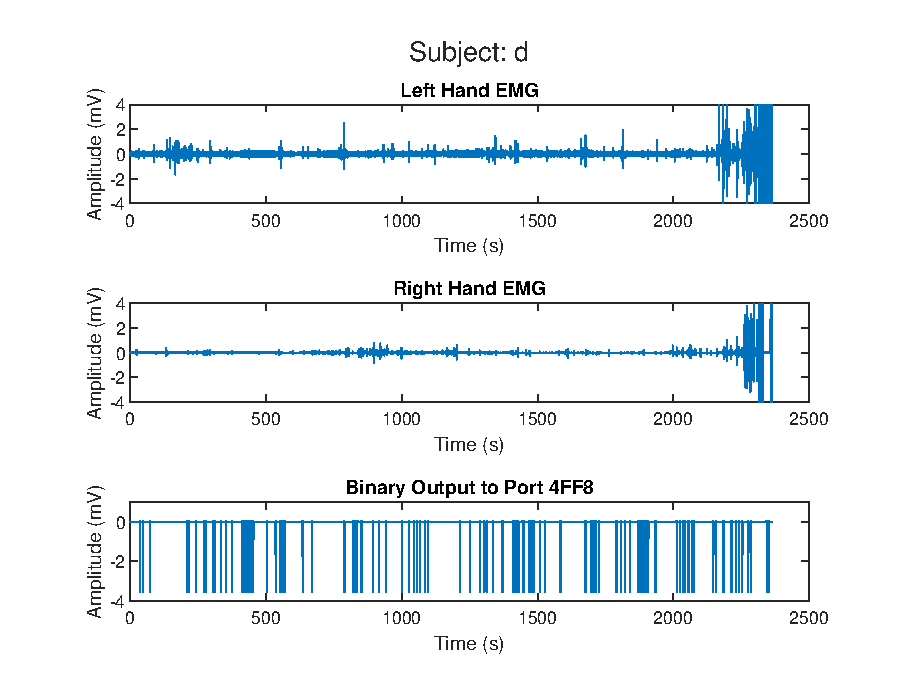
\includegraphics[width=0.75\linewidth]{figures/EMG_summary_d.eps}
    \caption{EMG Traces From Subject D's Trials}
    \label{fig:EMG_Sum_D}
\end{figure}
\begin{figure}[H]
    \centering
    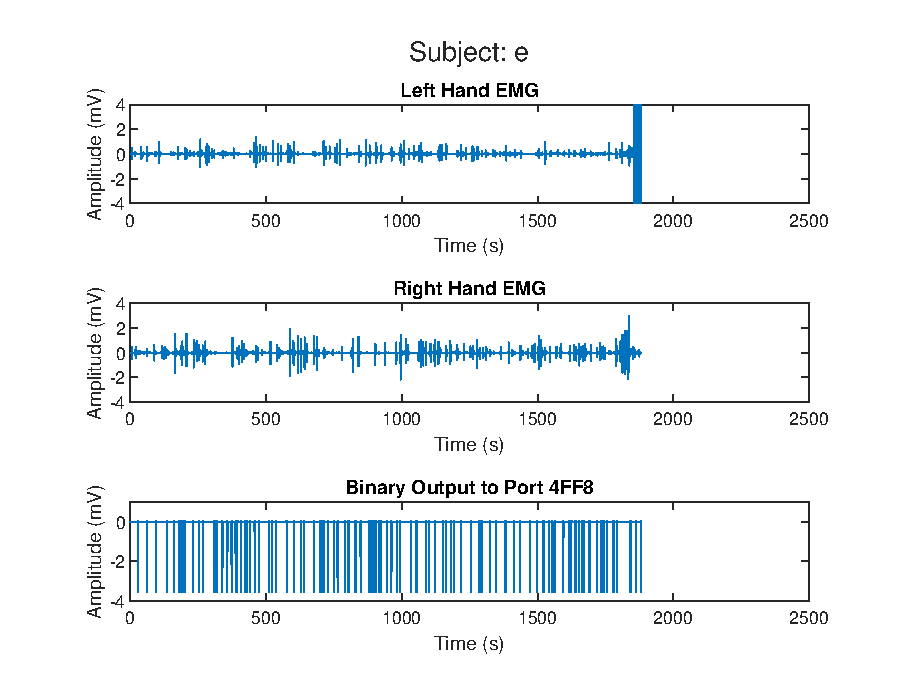
\includegraphics[width=0.75\linewidth]{figures/EMG_summary_e.eps}
    \caption{EMG Traces From Subject E's Trials}
    \label{fig:EMG_Sum_E}
\end{figure}
\begin{figure}[H]
    \centering
    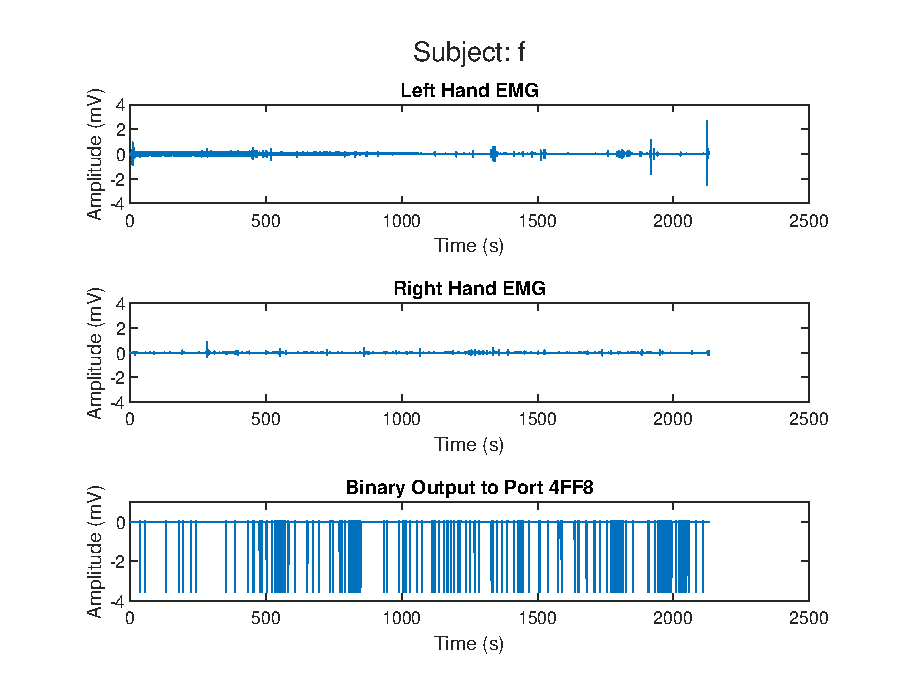
\includegraphics[width=0.75\linewidth]{figures/EMG_summary_f.eps}
    \caption{EMG Traces From Subject F's Trials}
    \label{fig:EMG_Sum_F}
\end{figure}

\section{EMG Trace - Task Relation Table}
\begin{table}[H]
    \begin{center}
        \caption{Tabulated Values of Trial Duration and EMG Duration}
        \label{tab:EMG_Relation_Table}
        \begin{tabular}{c|c|c|c}\hline
            EMG File & EMG Length (s) & Subject & Behavioural Data Length (s)\\\hline
            208     &   2245.99  & b & 2141.2 \\
            213     &   2331.07  & c & 2258.1 \\
            215     &   2364.20 &   d   &   2103.2\\
            217     &   1881.90 &   e   &   1568.5\\
            219     &   2132.39 &   f   &   2032.1\\\hline
        \end{tabular}
    \end{center}
\end{table}

\section{EMG Trace - Task Relation Plots}
\label{appendix:ExtraResults1_2}
\begin{figure}[H]
    \centering
    \includegraphics[width=0.75\linewidth]{figures/EMG_Trigger_Comparison_b}
    \caption{Output from EMG parallel port triggers related to Subject B's Trials}
    \label{fig:EMG_Trace_B}
\end{figure}
\begin{figure}[H]
    \centering
    \includegraphics[width=0.75\linewidth]{figures/EMG_Trigger_Comparison_c}
    \caption{Output from EMG parallel port triggers related to Subject C's Trials}
    \label{fig:EMG_Trace_C}
\end{figure}
\begin{figure}[H]
    \centering
    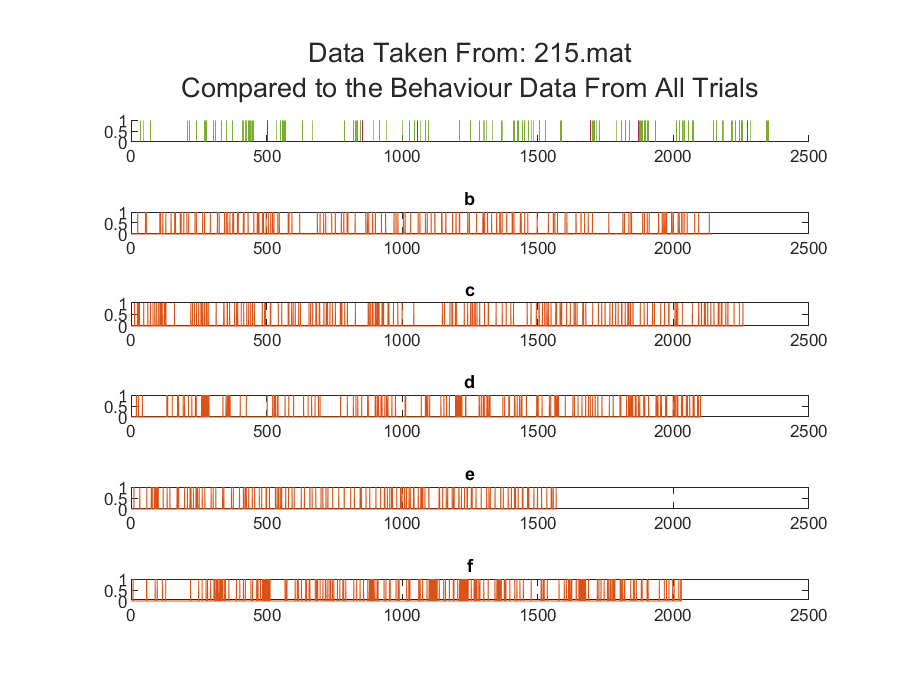
\includegraphics[width=0.75\linewidth]{figures/EMG_Trigger_Comparison_d}
    \caption{Output from EMG parallel port triggers related to Subject D's Trials}
    \label{fig:EMG_Trace_D}
\end{figure}
\begin{figure}[H]
    \centering
    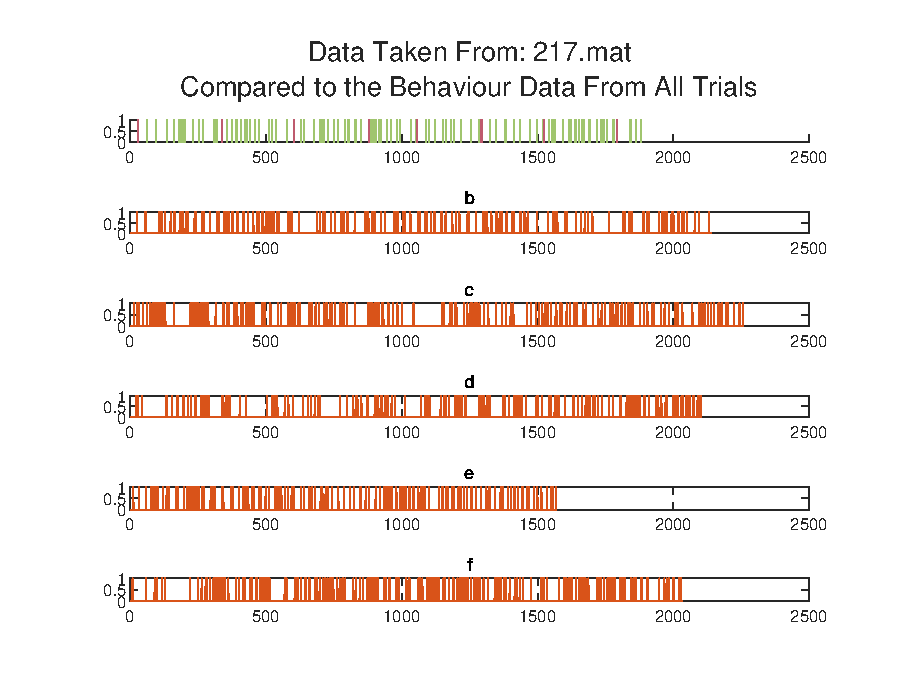
\includegraphics[width=0.75\linewidth]{figures/EMG_Trigger_Comparison_e}
    \caption{Output from EMG parallel port triggers related to Subject E's Trials}
    \label{fig:EMG_Trace_E}
\end{figure}
\begin{figure}[H]
    \centering
    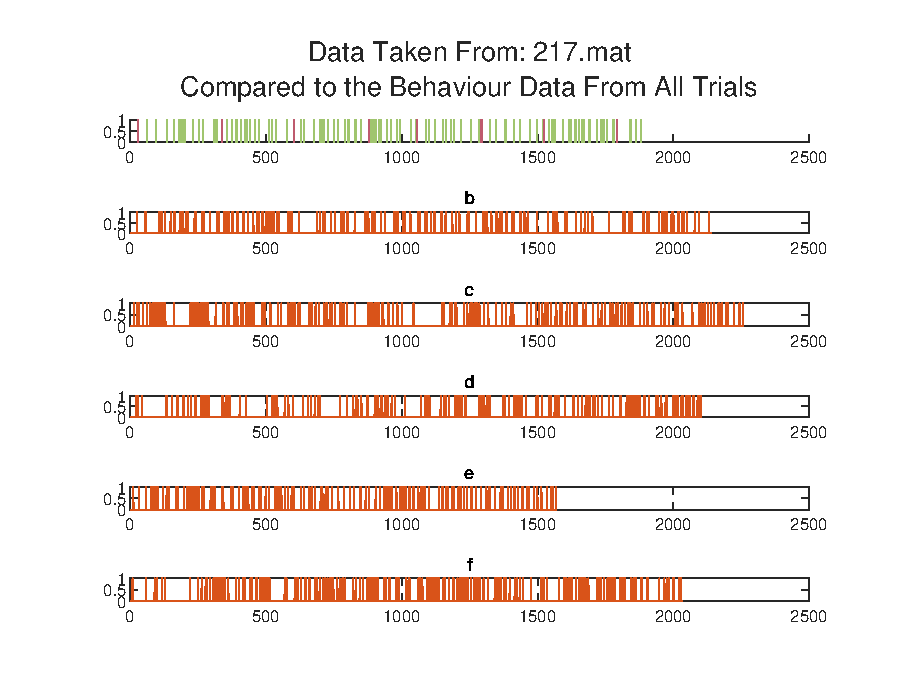
\includegraphics[width=0.75\linewidth]{figures/EMG_Trigger_Comparison_e}
    \caption{Output from EMG parallel port triggers related to Subject F's Trials}
    \label{fig:EMG_Trace_F}
\end{figure}

\end{appendices}